% to compile:
% bibtex project
% bibtex project
% pdflatex project

\documentclass[11pt]{article}
\usepackage{graphicx}
\usepackage{pdflscape}
\usepackage{amssymb}
\PassOptionsToPackage{hyphens}{url}\usepackage{hyperref}
\usepackage{listings}
\lstset{
basicstyle=\small\ttfamily,
columns=flexible,
breaklines=true
}
\usepackage{graphicx}
\graphicspath{ {./images/} }
\usepackage{csquotes}

\title{A Domain-Specific Knowledge Graph for Information Retrieval of News Items}
\author{Author: Christopher Eaves-Kohlbrenner \\ Supervisor: Michael Zakharyaschev}
\date{September 15, 2021}

\begin{document}
\maketitle

\begin{center}
\hfill \break
\hfill \break
\hfill \break
MSc Data Science project\\
Department of Computer Science and Information Systems\\
Birkbeck College, University of London\\
2021\\
\hfill \break
\hfill \break
\hfill \break

\textit{This report is substantially the result of my own work, expressed in my own words, except where explicitly indicated in the text. I have read and understood the sections on plagiarism in the Programme Handbook and the College web site. I give my permission for it to be submitted to the JISC Plagiarism Detection Service. \\
\hfill \break
The report may be freely copied and distributed provided the source is explicitly acknowledged.}
\end{center}

\newpage
\begin{abstract}
This project demonstrates how semantic technologies and natural language processing can produce a knowledge graph based on news articles. The result is twofold: a data pipeline for generating a knowledge graph from XML-formatted news articles and a proof-of-concept knowledge graph with relationships between news articles, entities, subjects, Wikidata, and more.

The proposed data pipeline may be of particular interest to data scientists or researchers in the knowledge graph space. The pipeline and code snippets demonstrate ingestion of text and XML documents into a graph database, natural language processing for named entity recognition and extraction, linked data with Wikidata and SPARQL, and Cypher queries for information retrieval in a Neo4j database.

The domain-specific news item knowledge graph is uniquely valuable for news industry practitioners. The knowledge graph exhibits how a large volume of news data--in this case 59,542 news items--can be queried for practical value as a journalist or media employee. The project documents queries that enable information retrieval of news items to support real-life use cases.

Finally, the reader is encouraged to run a demo version of pipeline and knowledge graph via the available code and sample data. The demo exhibits how users can interact with the proposed technologies to draw human insights over the data.


\end{abstract}

\newpage
\tableofcontents

\newpage
\section{Introduction}

\subsection{Background}
% [WIP] repurpose some proposal sections?
% similar to "A graph neural network path to network centralities.pdf"?
% % https://www.dcs.bbk.ac.uk/r/studentprojects/exampleprojects/msc/

The intent of this project is to build a knowledge graph for the news domain to improve news item recommendations and information retrieval. Knowledge graphs make use of the mathematical graph structure to enable knowledge representation or knowledge bases that can generate value in terms of human meaning.

News content is constantly generated by the media industry, providing a unique testing ground for knowledge graphs and their adjacent technologies, due the the volume and structure of journalistic news. Published news items are rich in content and facts, but are generally unstructured and semantically limited, only accessible as free text. This presents information retrieval challenges for news consumers and an opportunity for a domain-specific knowledge graph architecture.

The report that follows will present a specification for a news knowledge graph, demonstrate an example data extraction pipeline, and present the final proof of concept knowledge graph system. Furthermore, it will experiment with related semantic technologies like ontologies and linked data and natural language processing (NLP) for entity extraction and link prediction. The final outcome is a working software and database system with value to the end user and as an example of a technical architecture for media practitioners.

\subsection{Research Problem}

This project demonstrates the viability of a news information retrieval and recommendations system built with technologies including ontologies, linked data, and natural language processing. A proof-of-concept knowledge graph has been built using 59,542 items from the ``Reuters News Archive (30 Days)'' dataset\footnote{\url{https://aws.amazon.com/marketplace/pp/prodview-qwmkdffmmjesa}}, to illustrate how information can be extracted from published news items and ingested into a knowledge graph. The end result is a knowledge graph which can be queried by an end user or can recommend a similar item of interest based on an item the user is reading.

As outlined in the project proposal\cite{ek-proposal}, the \textit{aims} include:
\begin{itemize}
  \item Design and implement a system for news information retrieval and recommendations
  \item Determine whether and how certain technologies, including knowledge graphs, ontologies, linked data, and natural language processing, can be used to implement such a system
\end{itemize}

The \textit{objectives} or concrete and verifiable outcomes include:
\begin{itemize}
  \item Develop a software specification for the design and implementation of an information retrieval system for news XML documents
  \item Build a data extraction pipeline for ingesting news data into the system
  \item Build a knowledge graph prototype stored in Neo4j and query-able via Cypher
  \item Experiment with semantic technologies and natural language processing for entity extraction and link prediction to enhance the knowledge graph
\end{itemize}

[WIP](Note to self: check back against proposal aims and objectives before finishing this section)

\subsection{Benefits and Use Cases}
The proposed pipeline and resulting knowledge graph are of particular value to two user types:

\textbf{Journalists and media companies} can use this pipeline to store all news items when published. This has the following benefits:
\begin{enumerate}
  \item{
    \textit{Context}: Journalists can view deeper context when writing and researching a story.

    For example, a journalist reporting on Austria may be interested in some background context and learn, via the Wikidata ontology, that Austria is an instance of landlocked country, Rechtsstaat, and other categories.
  
    \centerline{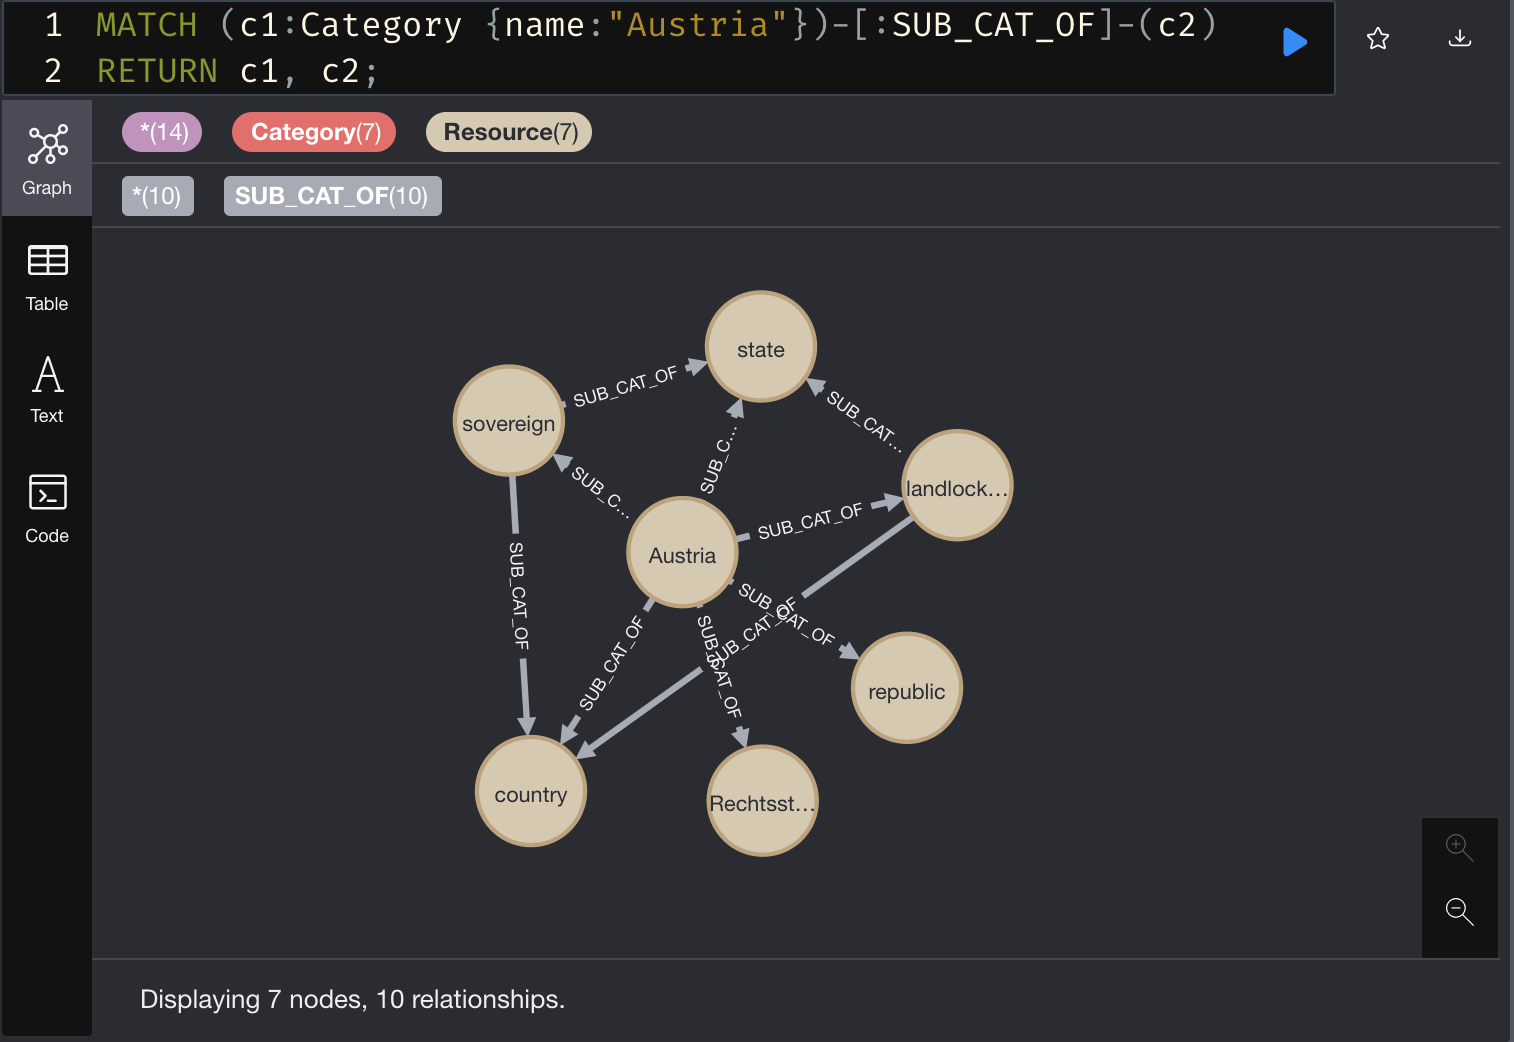
\includegraphics[scale=0.3]{use-case-1a}}

    From there, she may seek to draw links to other similar categories and learn that Senegal, Brazil, and Transnistria\footnote{A ``de facto unrecognized state in Eastern Europe that has declared independence from Moldova''. (\url{https://www.wikidata.org/wiki/Q907112})} are also instances of Rechtsstaat.
  
    \centerline{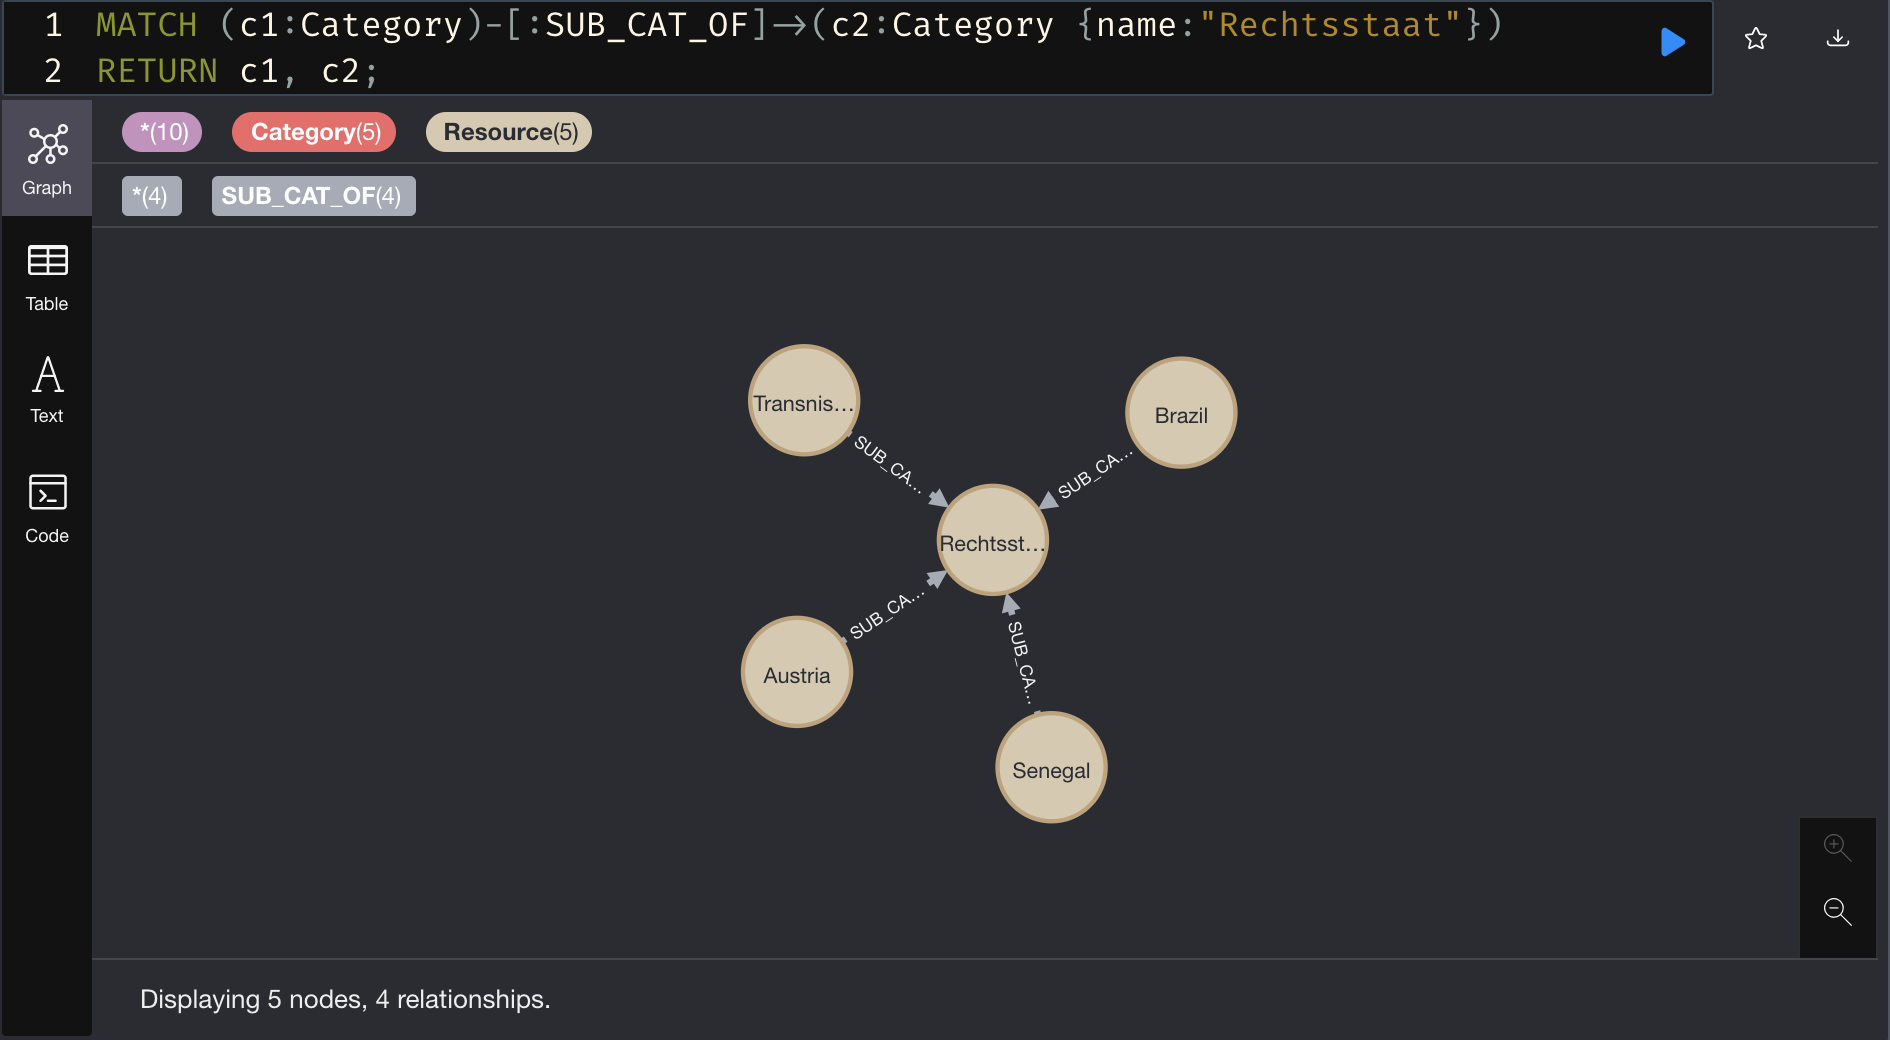
\includegraphics[scale=0.3]{use-case-1b}}

    Finally, she may be deepen her contextual knowledge by viewing any news items previously published about countries in a category like Rechtsstaat\footnote{A ``doctrine in European legal thinking, means `state based on justice and integrity'.'' (\url{https://www.wikidata.org/wiki/Q4209223})}.
  
    \centerline{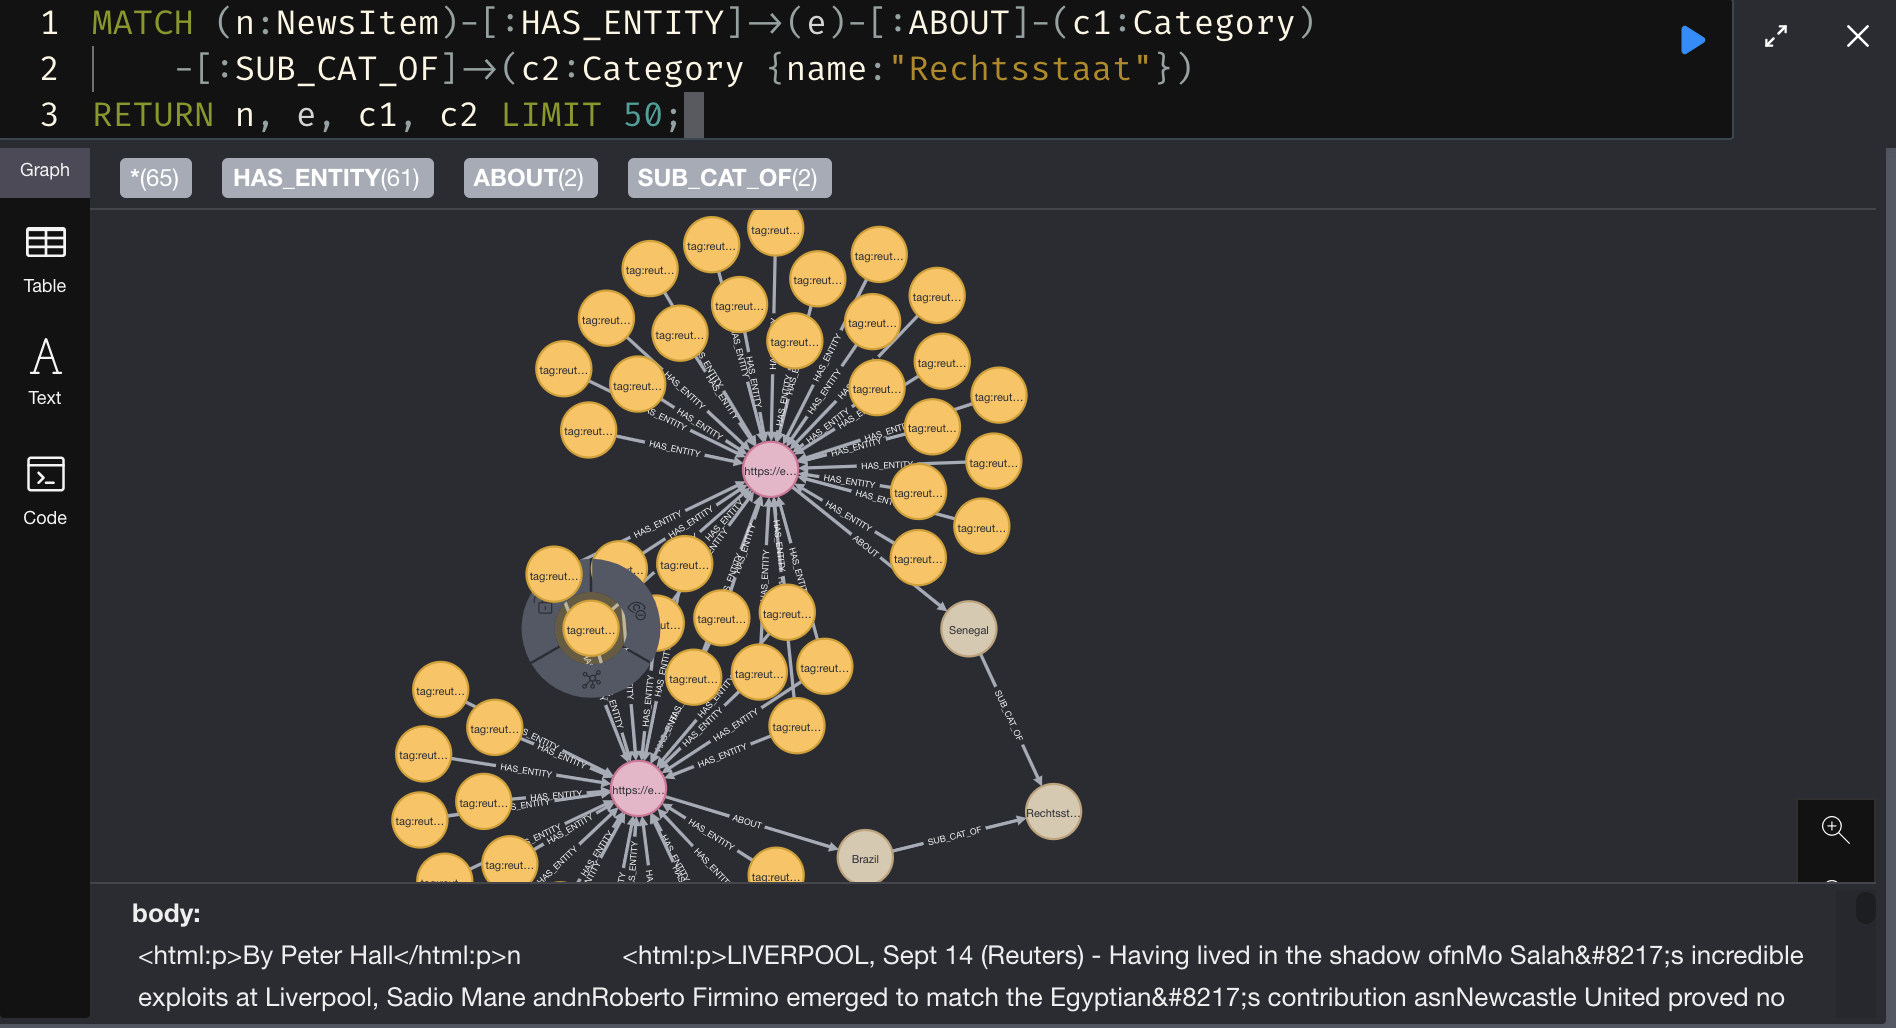
\includegraphics[scale=0.3]{use-case-1c}}
  }
  \item{
    \textit{Recommendations}: Media companies can leverage the knowledge graph as an API to provide recommendations to customers based on items they are viewing. This provides an improved user experience and increases the time the customers remain on the company's platform, thus increasing company revenue.

    For example, a customer may be reading a news article about football:

    \centerline{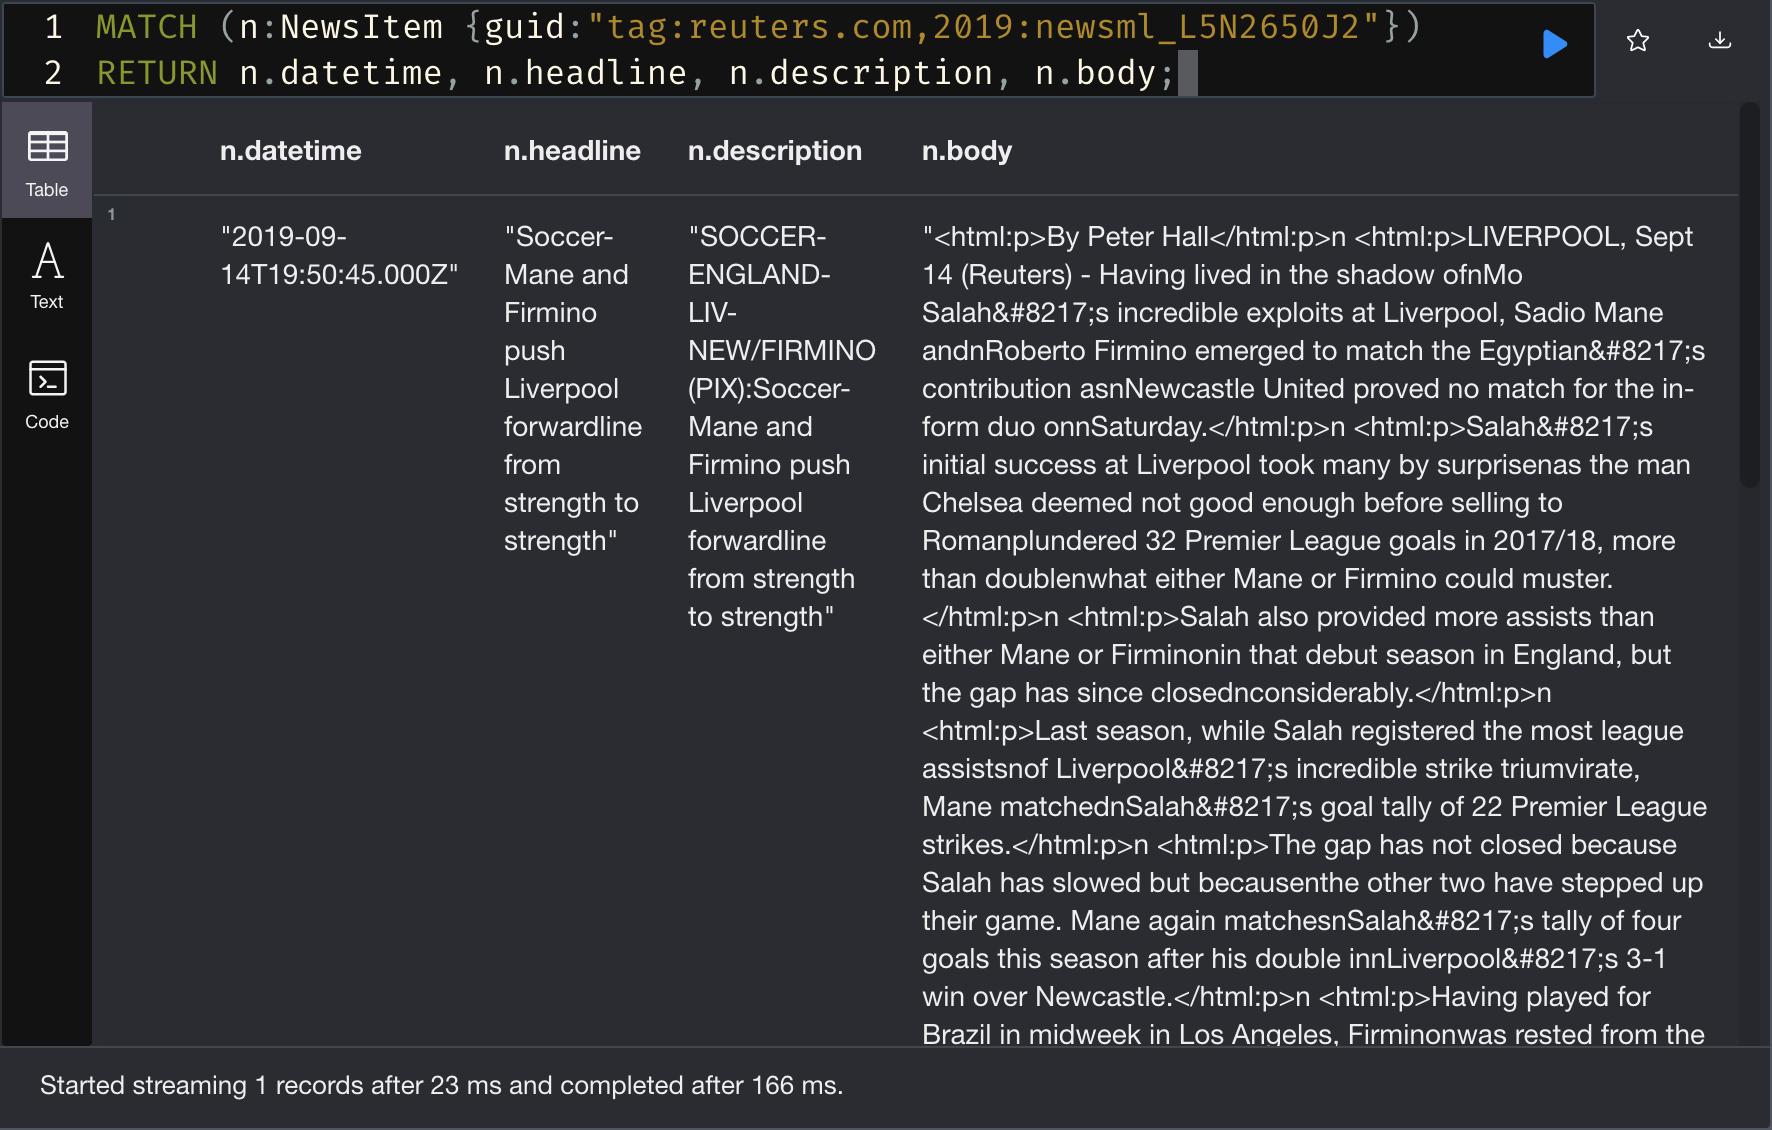
\includegraphics[scale=0.3]{use-case-2a}}

    The knowledge graph provides an easy way for the customer to view ``similar'' articles, by retrieving other articles that share knowledge graph paths to relevant football players:
    
    \centerline{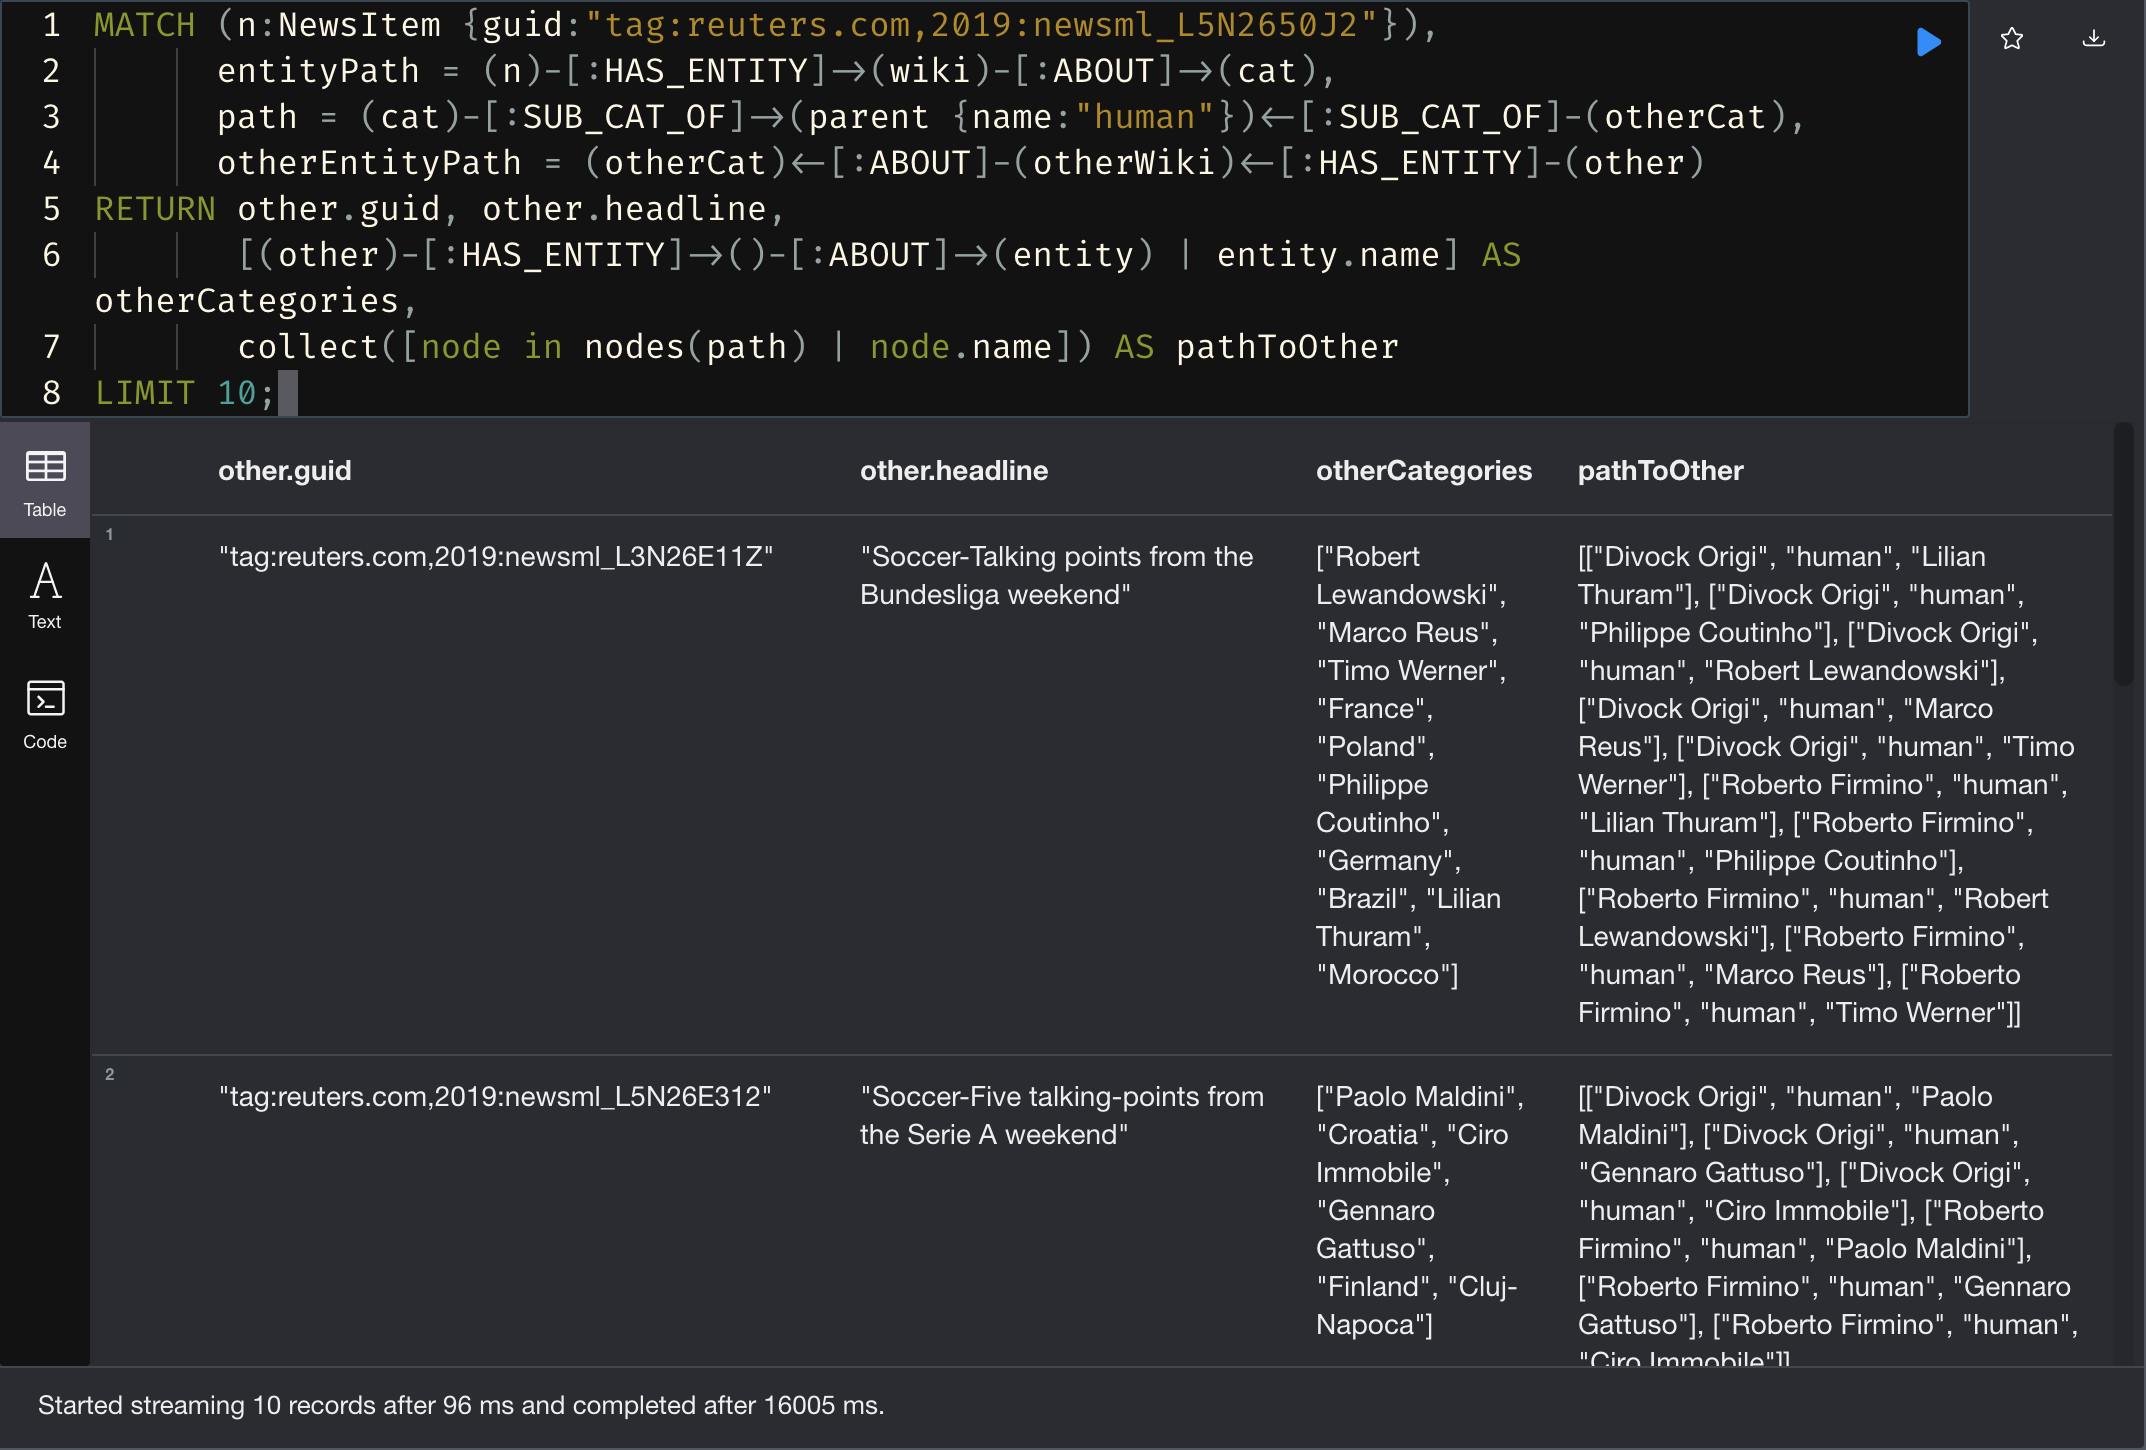
\includegraphics[scale=0.25]{use-case-2c}}
    }
\end{enumerate}

The second user type who would benefit from this pipeline and knowledge graph are \textbf{researchers and media customers}, who can use the knowledge graph for information retrieval and data mining. For example, the knowledge graph adds structure to semi-structured documents and draw meaning from the text in the following ways:
\begin{enumerate}
  \item{
    \textit{Entity extraction}: Entities have been extracted for each news item, enriching the news items' metadata and enabling users to identify the entities in a news item or news items about a given entity. A given news item's entities can be ranked based on their salience, giving an idea of each entity's relevance:

    \centerline{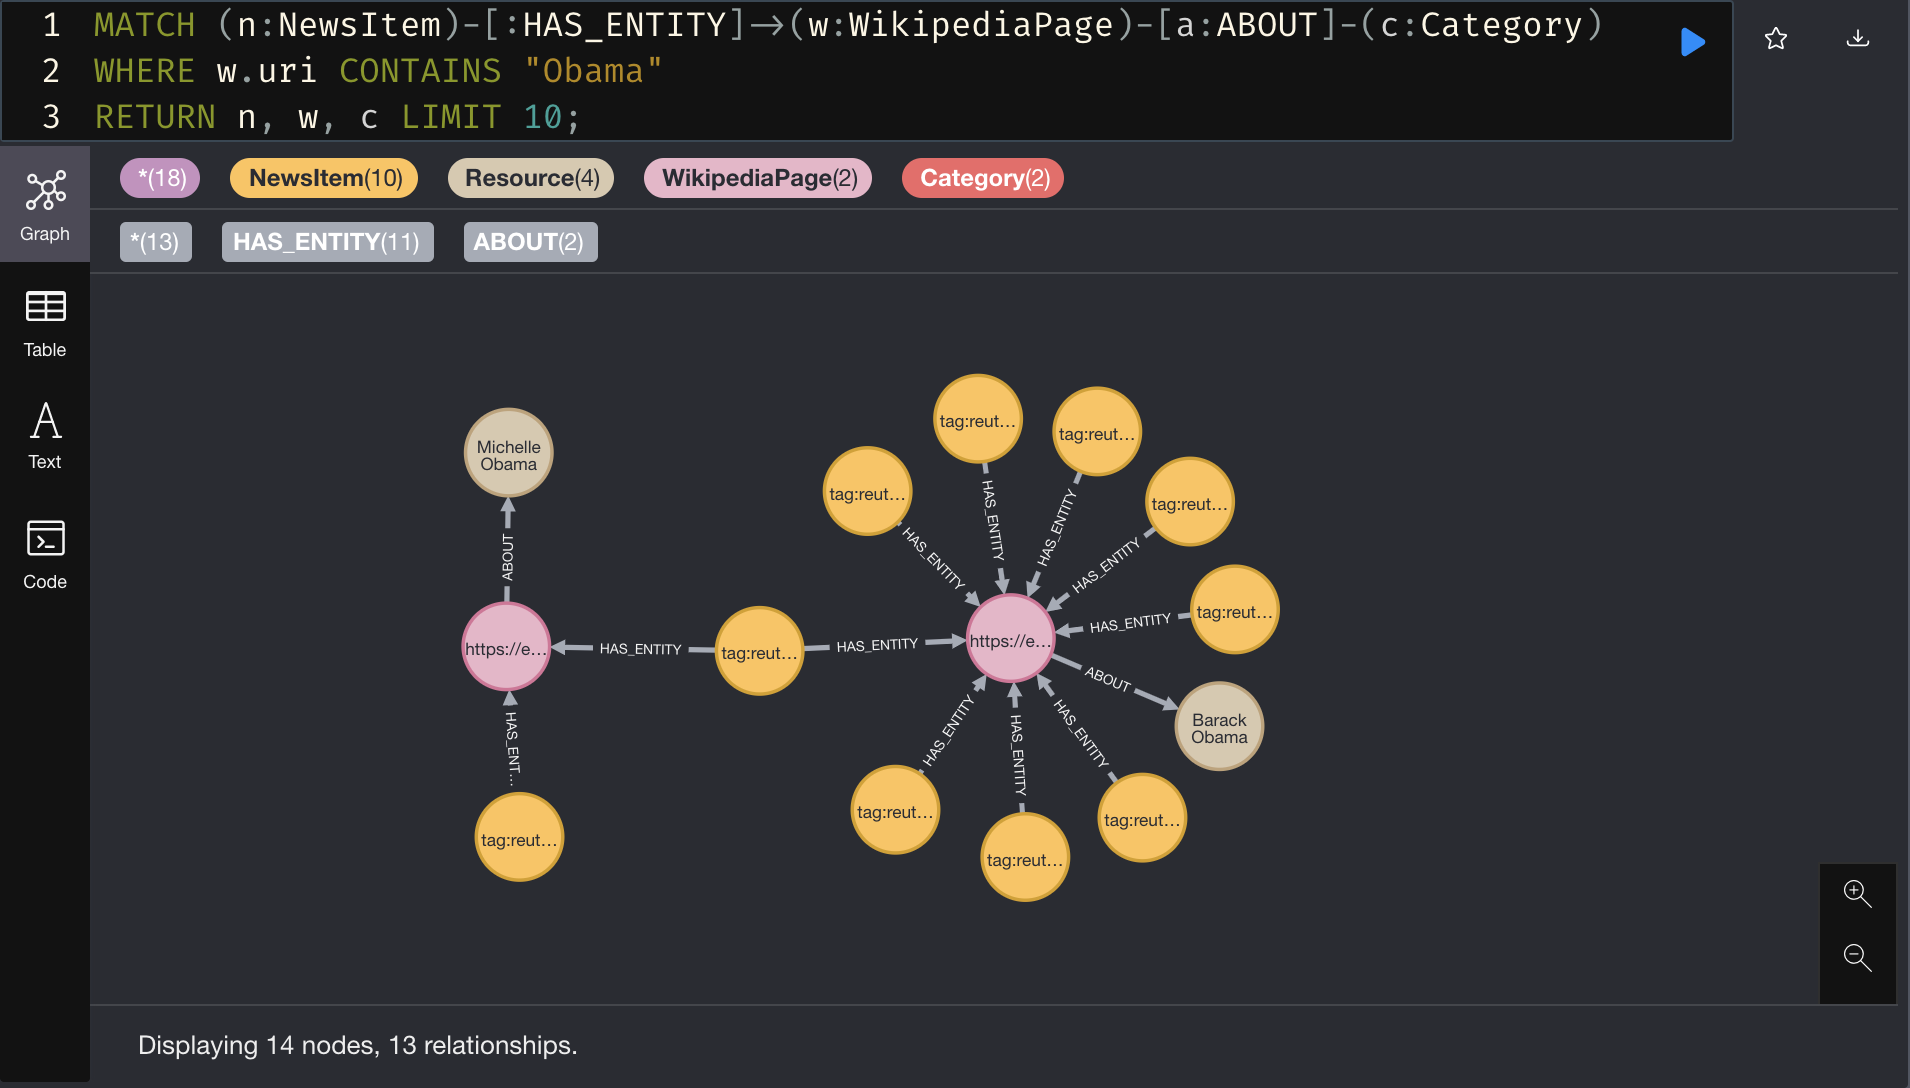
\includegraphics[scale=0.3]{use-case-3a}}
    \centerline{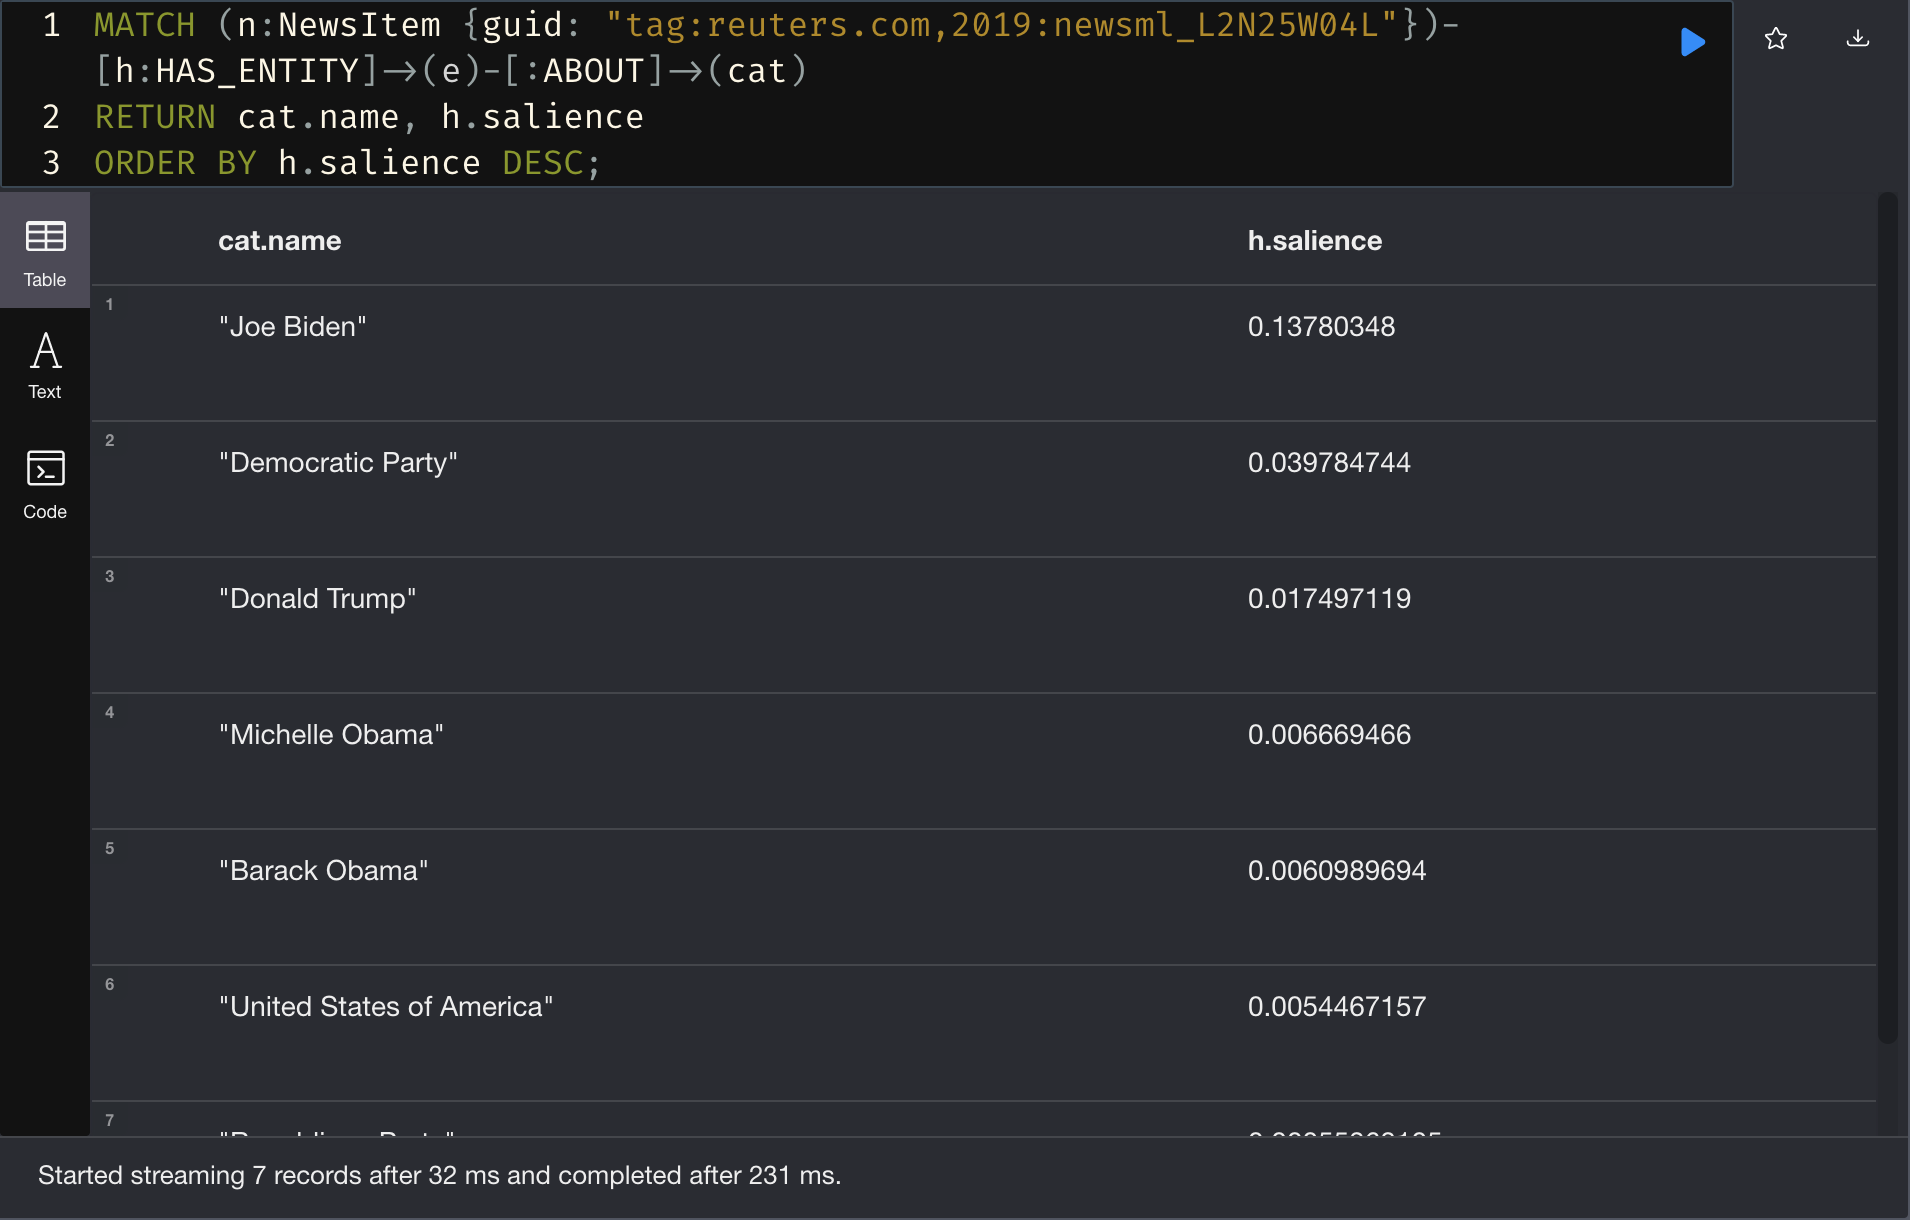
\includegraphics[scale=0.3]{use-case-3b}}

  }
  \item{
    \textit{Similarity}: News items can be similar based on shared relationships, as well as graph properties like K-nearest neighbours, Euclidean distance, or cosine similarity. As a simple example, Jaccard similarity can be computed using shared entities or subjects:

    \centerline{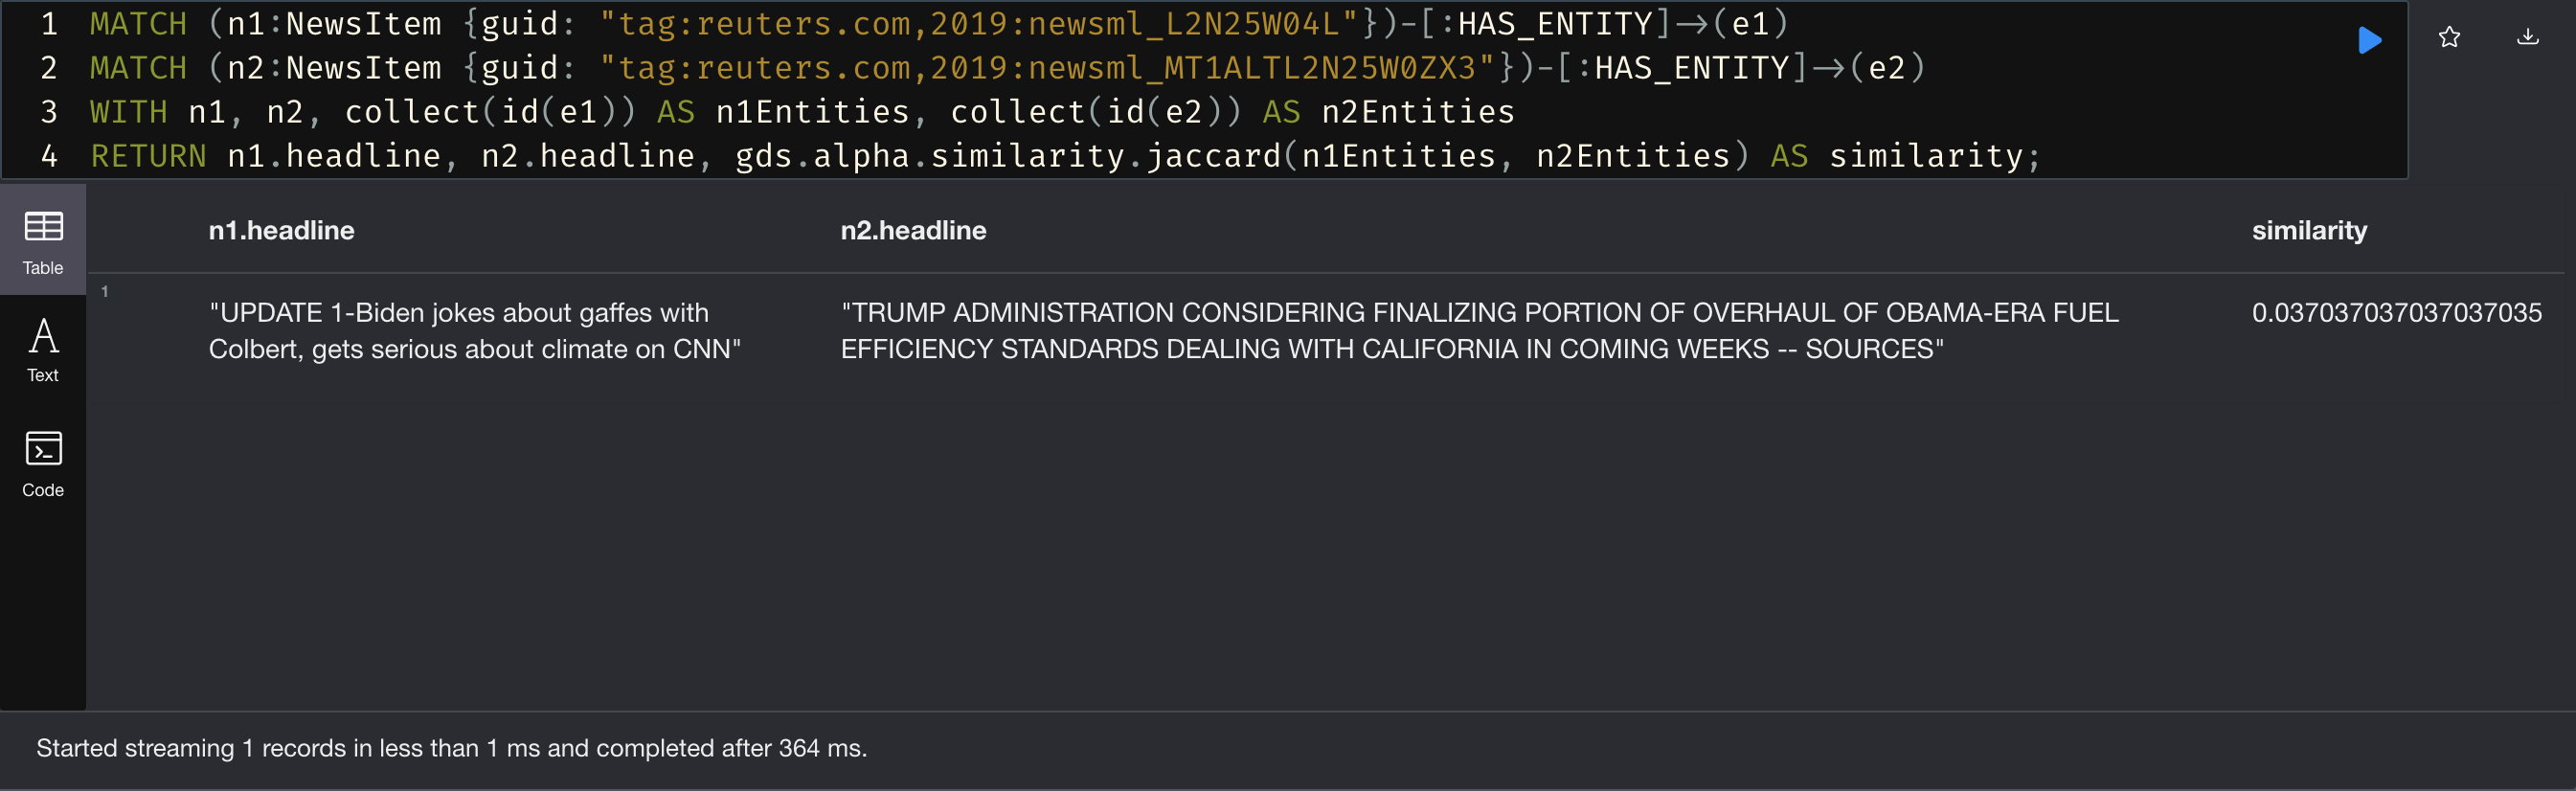
\includegraphics[scale=0.3]{use-case-4-similarity-1}}
  
    \centerline{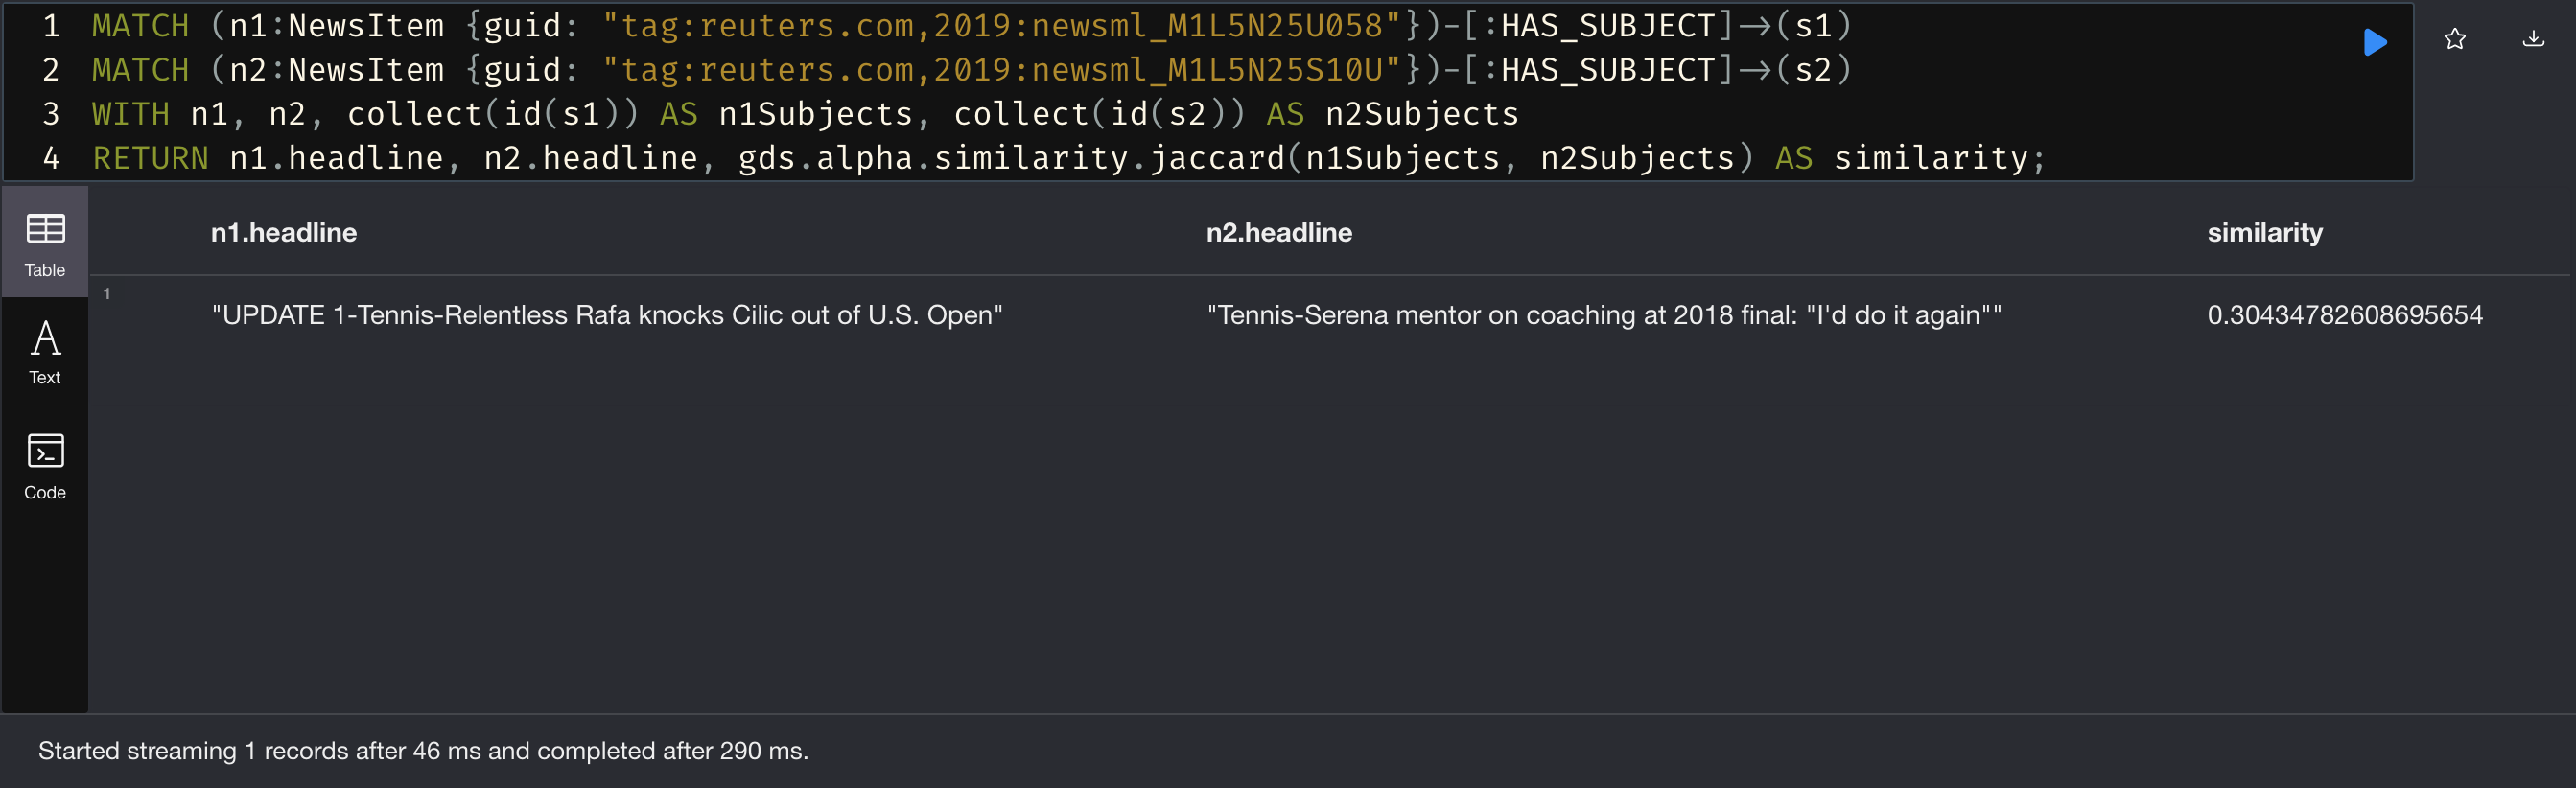
\includegraphics[scale=0.3]{use-case-4-similarity-2}}
  
    \centerline{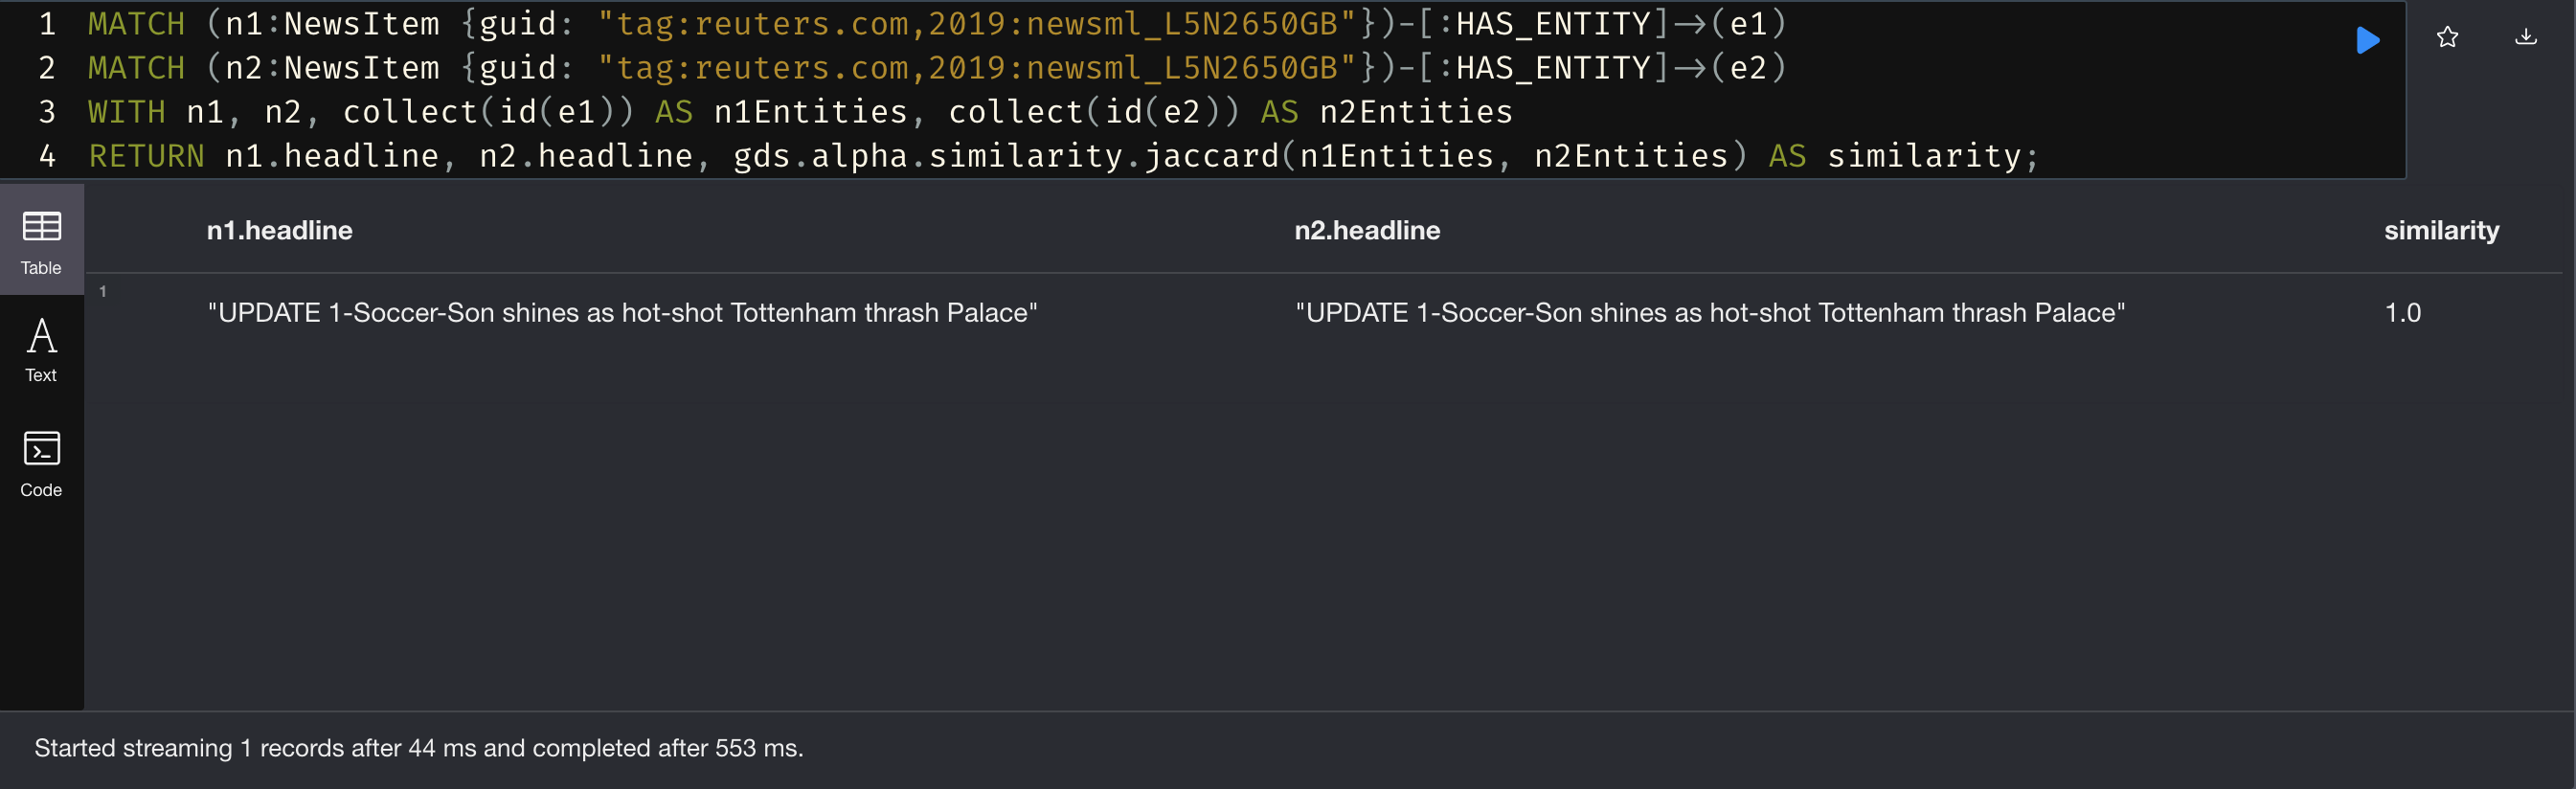
\includegraphics[scale=0.3]{use-case-4-similarity-3}}
  }
  \item{
    \textit{Categorisation}: By linking data with Wikidata, particularly Wikidata's ontology of categories and subcategories, the news items can be categorised in new ways. For example, categories enable unique queries like ``all articles featuring landlocked countries'' and provide additional details about companies like IBM as a public company, technology company, etc.:

    \centerline{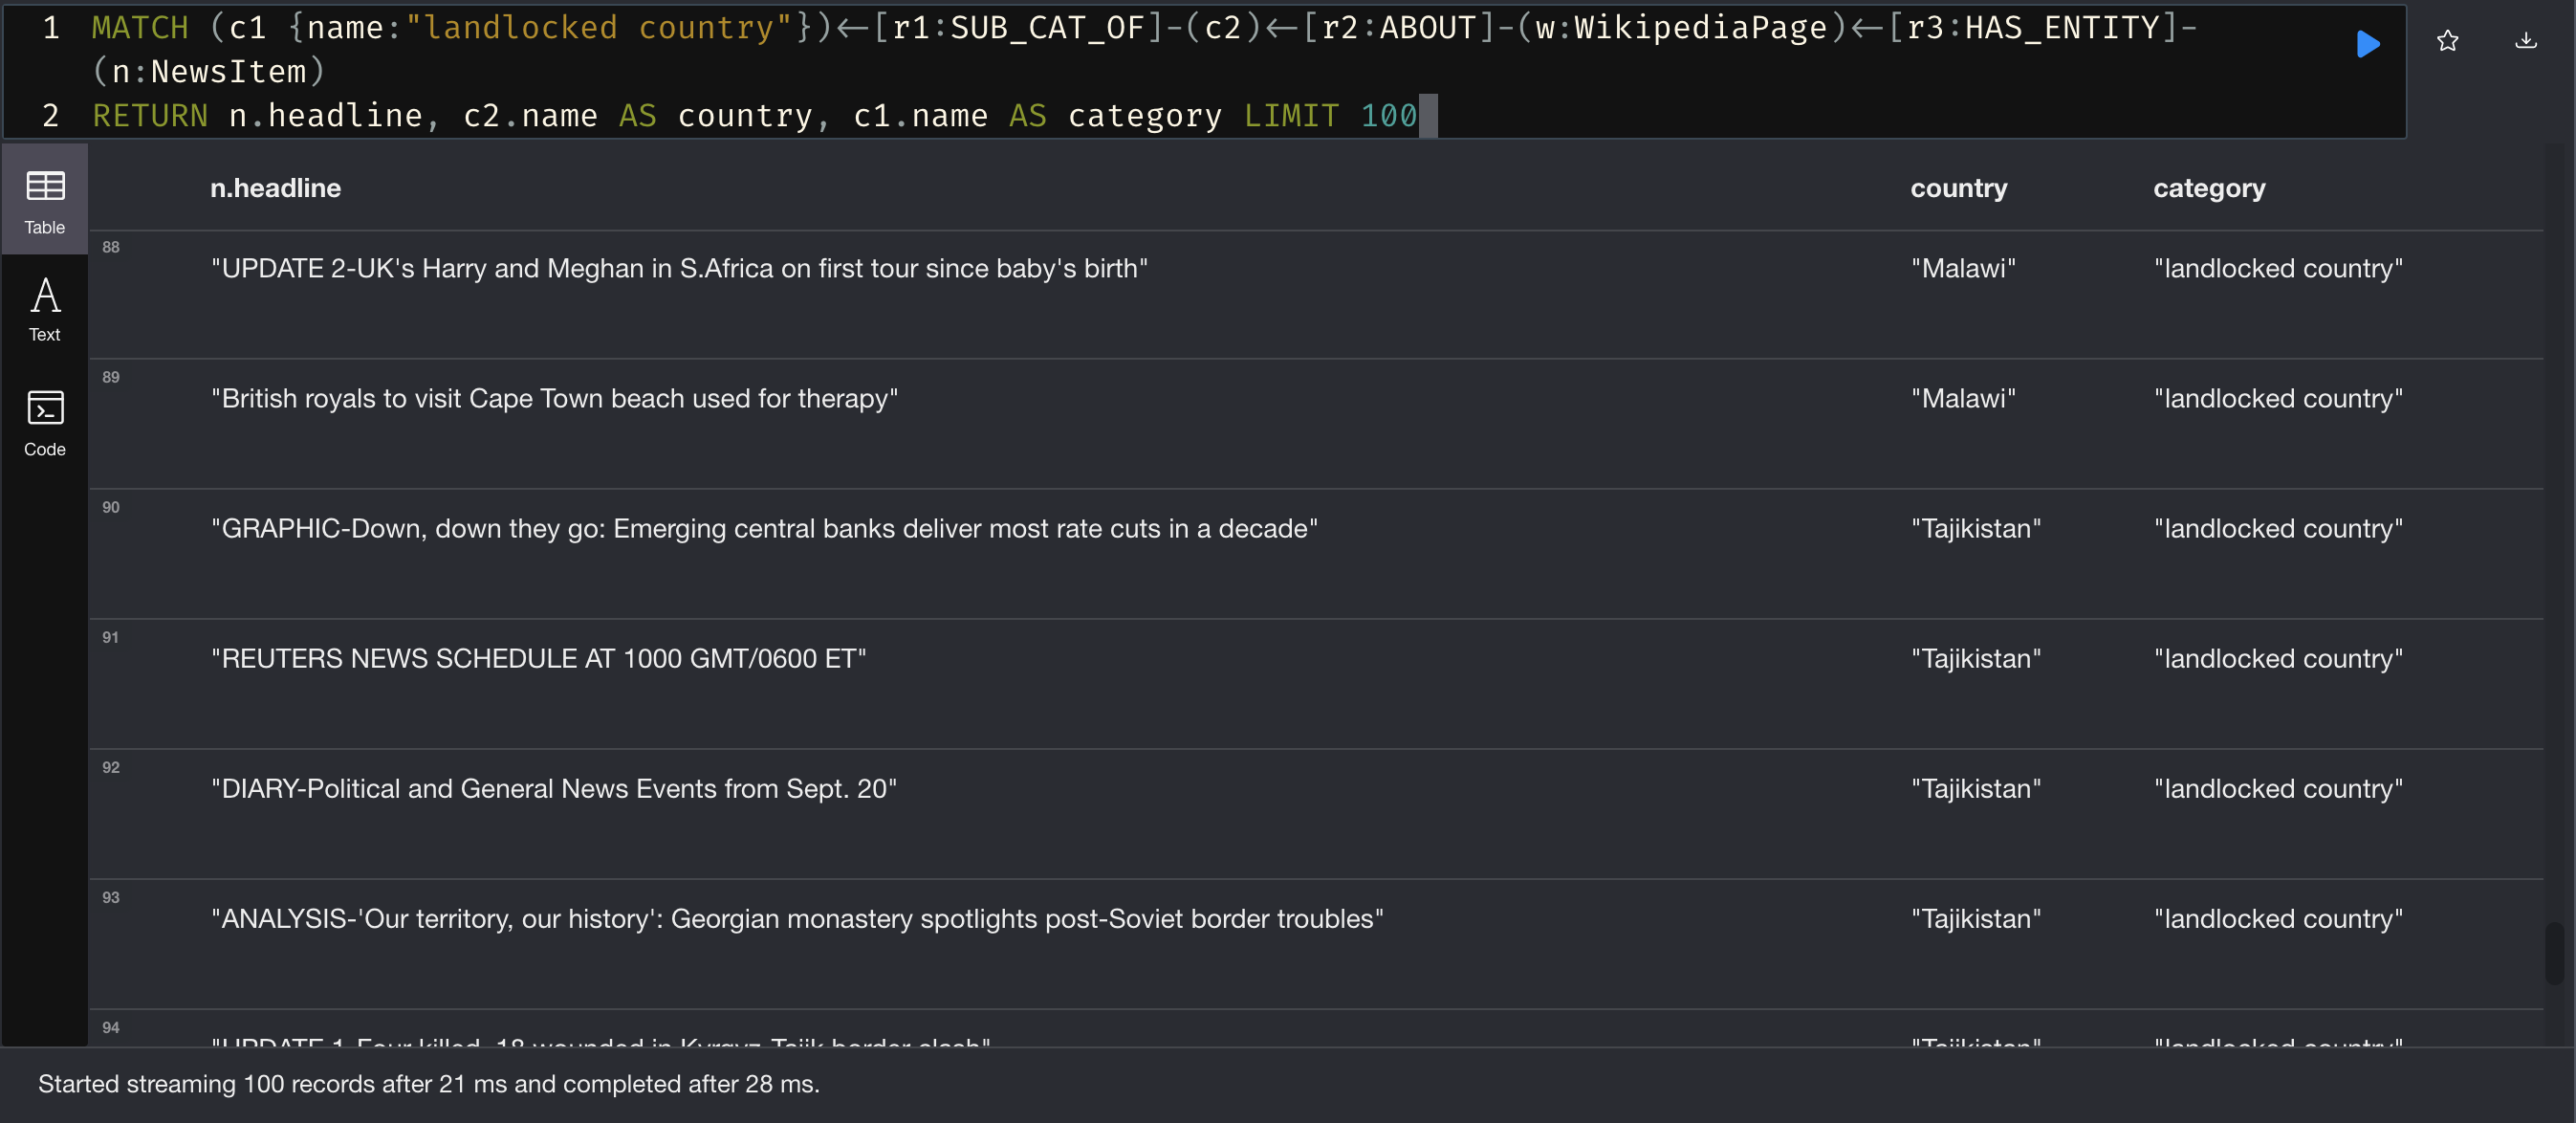
\includegraphics[scale=0.3]{use-case-5a}}

    \centerline{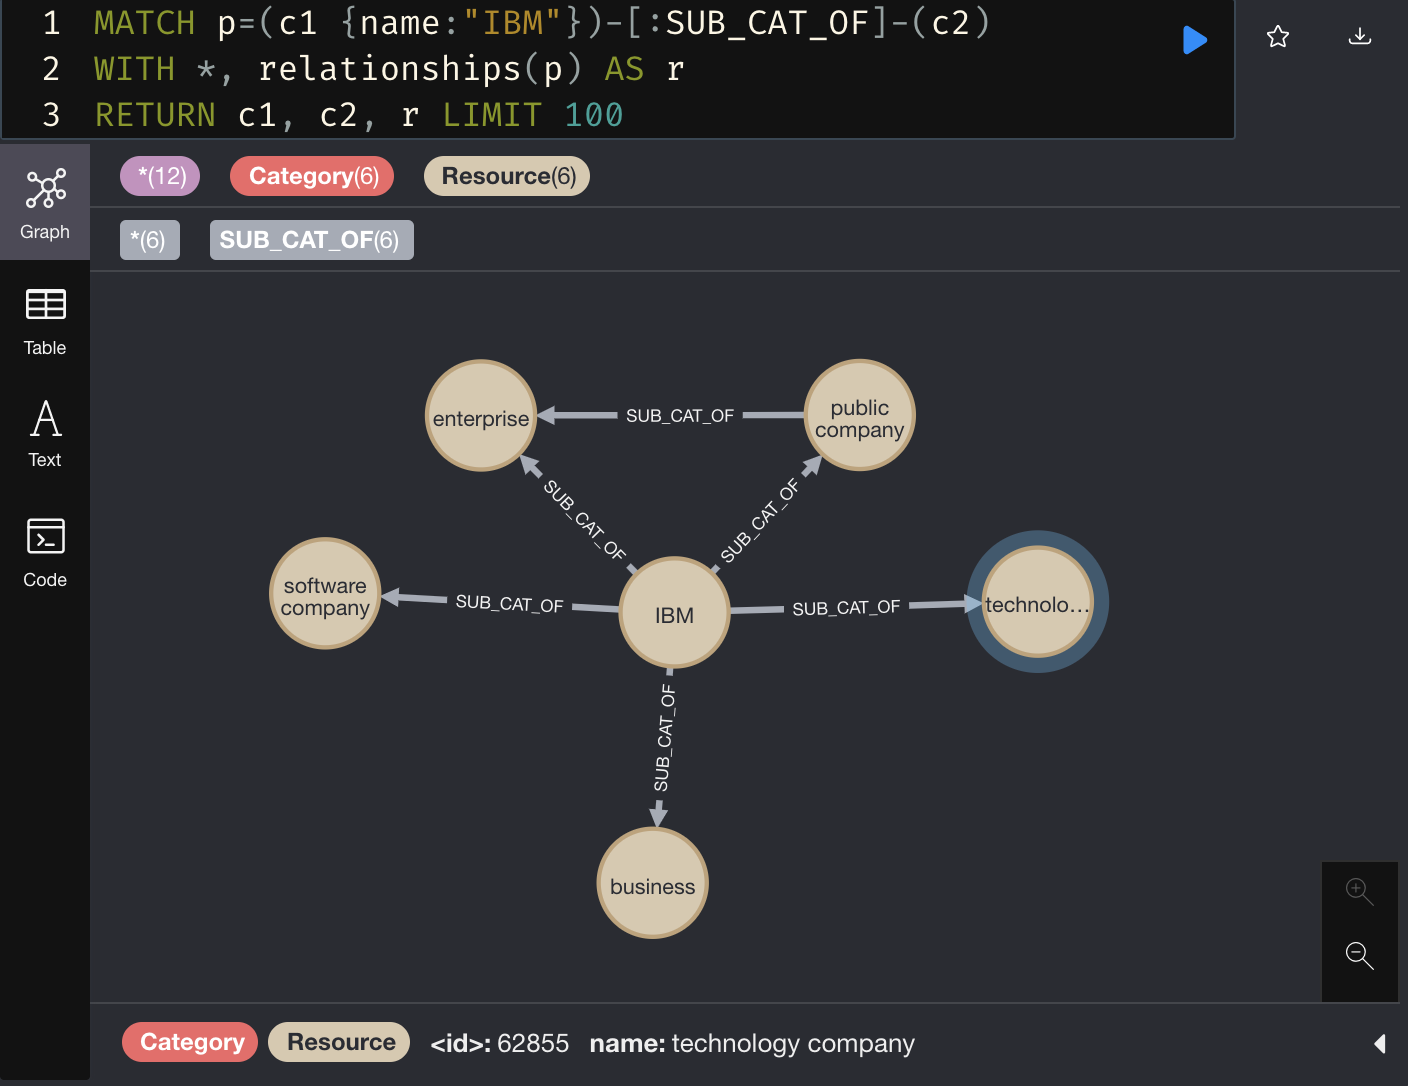
\includegraphics[scale=0.3]{use-case-5b}}
    }
\end{enumerate}


\newpage


\section{Literature Review}

\label{sec:LiteratureReview}

  \subsection{News Media Knowledge Systems}

  As reviewed in the project proposal\cite{ek-proposal}, a number of knowledge representation systems have been proposed or built in the media industry as news-specific systems for the aggregation, generation, or linking of news articles. 

  \begin{figure}
    \centerline{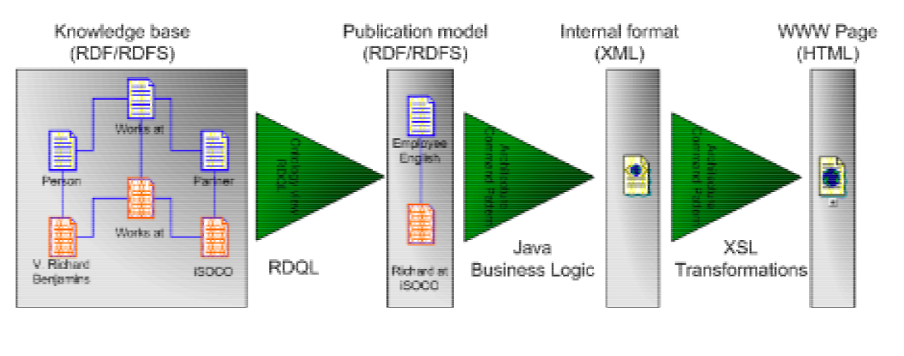
\includegraphics[scale=0.4]{literature-review--neptuno.png}}
    \caption{\textit{Neptuno publication workflow}}
  \end{figure}

  The first system of note historically is \textit{Neptuno} (2004)\cite{castells2004neptuno}, which introduces ``emergent semantic-based technologies to improve the processes of creation, maintenance, and exploitation of the digital archive of a newspaper''. This archive-focused technique presents useful background for this project, but is oriented as an ontology-first approach. For example, Neptuno's ``Publication through visualisation ontology'' model begins with RDF and ends with XML and HTML, whereas this project begins with published XML documents (see ``Figure 1'').

  \begin{figure}
    \centerline{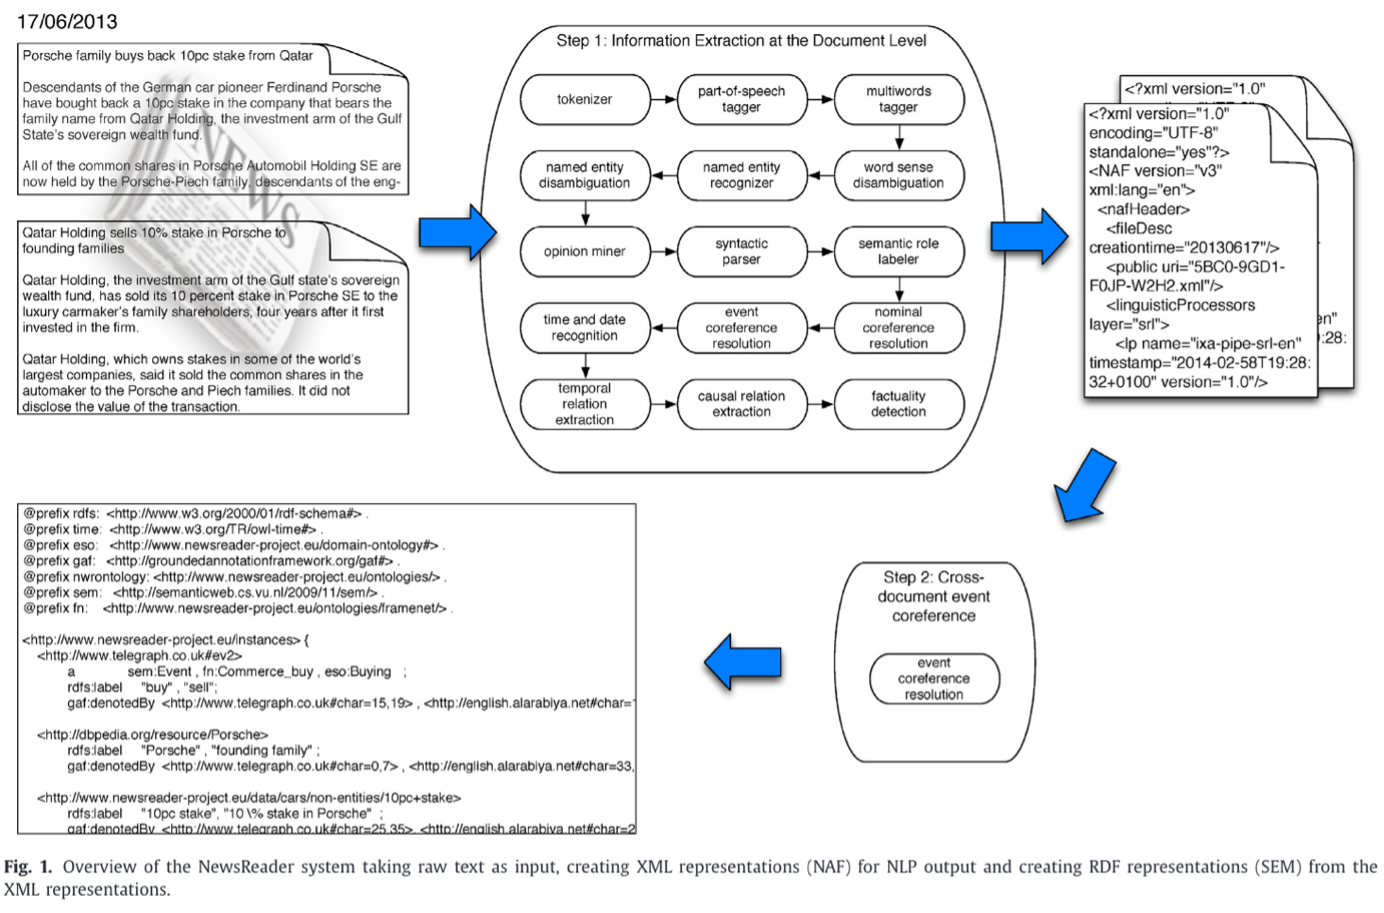
\includegraphics[scale=0.4]{literature-review--newsreader.png}}
    \caption{\textit{NewsReader workflow from XML to RDF representation}}
  \end{figure}

  Meanwhile, \textit{News Engine Web Services (NEWS)} \cite{fernandez2010news} (2010), \textit{NewsReader} \cite{vossen2016newsreader} (2016), and \textit{Acquisition de Schémas pour la Reconnaissance et l'Annotation d'Événements Liés (ASRAEL)} \cite{rudnik2019searching} (2019) each approach the news industry from a semantic technology point of view, using ontology, metadata vocabularies, RDF, and Wikidata. NewsReader, for example, matches the sequence of operations that this project proposes, from raw text to information extraction, linked data, and ontology development (see ``Figure 2'').

  \begin{figure}
    \centerline{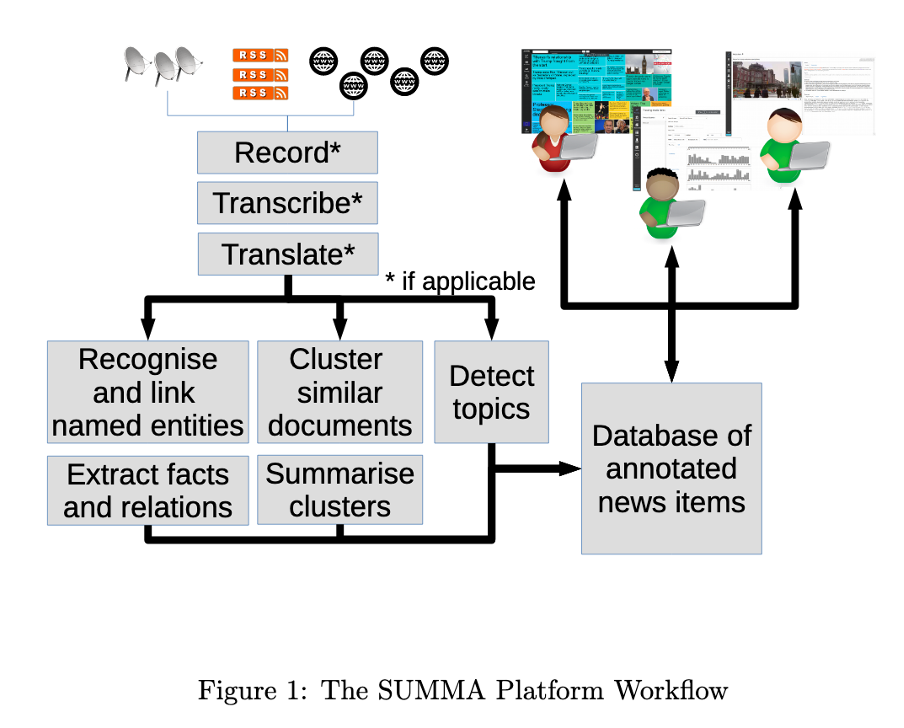
\includegraphics[scale=0.4]{literature-review--summa.png}}
    \caption{\textit{SUMMA platform workflow}}
  \end{figure}

  Two recent efforts have applied natural language processing and machine learning techniques to news data. These are \textit{Scalable Understanding of Multilingual MediA (SUMMA)} \cite{germann2018integrating} (2018) and \textit{News Hunter} \cite{berven2020knowledge} (2020), which are both platforms and architectures for news monitoring and applying NLP pipelines. For example, SUMMA matches the general data flow proposed in this project (see ``Figure 3''). Furthermore, it presents useful state of the art for NLP techniques, including entity extraction, clustering, and topic detection, which will be pursued in this project.

  \begin{figure}
    \centerline{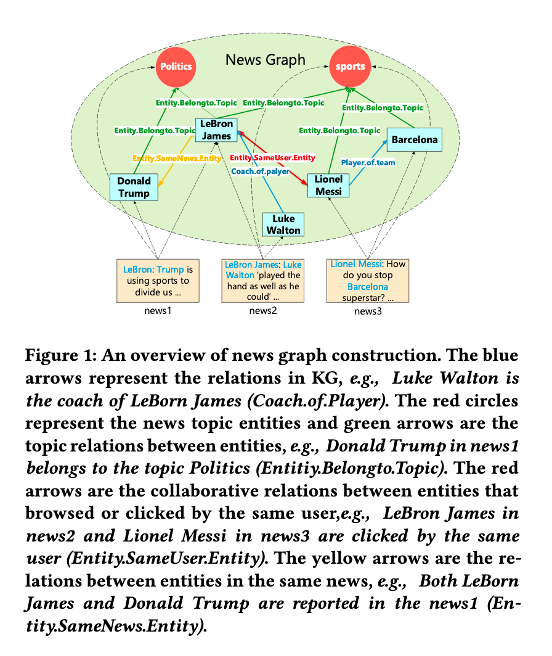
\includegraphics[scale=0.4]{literature-review--newsgraph.png}}
    \caption{\textit{News Graph sample construction, including relationships between entities and news topics}}
  \end{figure}

  \textit{News Graph} \cite{liu2019news} (2019), may be the research most directly relevant to this project. As an enhanced news knowledge graph that adds new entities and relationships and removes news-irrelevant links, it models the desired outcome of news recommendations based on the application of NLP techniques. On the other hand, it focuses on mathematical techniques around entity embeddings for news recommendations; this is of note for the project, but goes deeply into a specific direction rather than as a general knowledge graph in the news domain.

  Finally, a number of other systems were reviewed, but deemed not relevant to the project at hand. These include \textit{Global Database of Events, Language, and Tone (GDELT)}\footnote{\url{https://www.gdeltproject.org/}} (2013) and \textit{Event Registry} \cite{leban2014event} (2014), which were proposed as real-time monitoring systems for analysing ``world events'' or ``world's news media''. These both approach the field differently, as a high-volume monitoring system rather than a knowledge graph architecture for information retrieval. Furthermore, \textit{NewsAPI}\footnote{\url{https://newsapi.org/}} (2017) is JSON API to retrieve articles and breaking news headlines from various sources, but not an overall knowledge architecture. Finally, \textit{Reuters' Tracer} \cite{liu2017reuters} (2017) ``automates end-to-end news production using Twitter data.'' It provides an interesting example of a data pipeline, but with a different use case.

  \subsection{Knowledge Graphs}

  In addition to the literature on news-specific knowledge systems, there is a wealth of resources related to knowledge graph architecture more broadly. For example, \textit{Architecture of knowledge graph construction techniques} (2018) \cite{zhao2018architecture} presents a helpful distinction between two types of knowledge graph approaches:

  \begin{displayquote}
  In the top-down approach emphasizing the well-defined domain ontologies, the domain ontologies and their schema should be defined at first, and then [...] knowledge instances are added into knowledge base. The bottom-up approach extracts knowledge instances from knowledge resources. After knowledge fusing the populated instances, the top-level ontologies are built by means of knowledge instances to create the whole KGs.
  \end{displayquote}

  This clarifies that the news domain knowledge graph proposed in this project takes a bottom-up approach, starting from the text data and building up to entity extraction and ontologies.

  Two other useful resources are \textit{A review of relational machine learning for knowledge graphs} \cite{nickel2015review} and \textit{Knowledge graph embedding: A survey of approaches and applications} \cite{wang2017knowledge}, which review the application of relational machine learning and graph embedding in the knowledge graph domain. These techniques are out of scope for this effort, but present interesting opportunities for future research.

\section{Technical Specifications}

  \begin{figure}
  \centerline{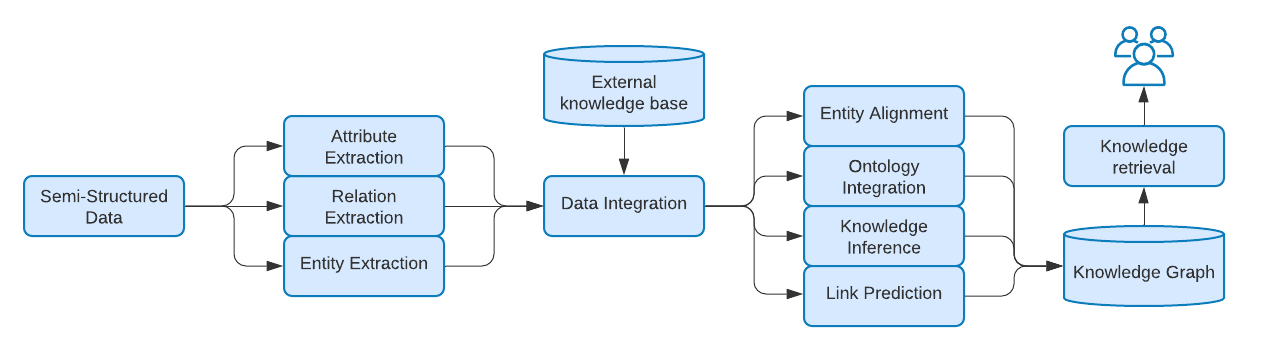
\includegraphics[scale=0.275]{bottom-up-kg-architecture}}
  \caption{\textit{Architecture of the bottom-up knowledge graph}}
  \label{figure:BottomUpKGArchitecture}
  \end{figure}

  As initially proposed\cite{ek-proposal}, the bottom-up architecture will take as input the semi-structured data in the form of XML documents, extract entities, attributes, and relations, and integrate these with additional data to produce a knowledge graph. See ``Figure 5'' for a depiction of the data pipeline architecture.

  \subsection{Input / Output}
  This project proposes a \textit{data pipeline} to transform XML or raw text news items into a \textit{knowledge graph}. For example, given an \textbf{input} of XML documents in the following format (\textit{\textbf{Demo file available on Github}}\footnote{\lstinline{00_tag:reuters.com,2019:newsml_L2N25V1DP:702697965.XML} (\href{https://github.com/Birkbeck/msc-data-science-project-2020_21---files-heychrisek/}{full code on Github})}):
  \begin{lstlisting}[basicstyle=\tiny]
  <?xml version=``1.0'' encoding=``UTF-8''?>
  <newsMessage xmlns=``http://iptc.org/std/nar/2006-10-01/'' xmlns:rtr=``http://www.reuters.com/ns/2003/08/content'' xmlns:x=``http://www.w3.org/1999/xhtml'' xmlns:xsi=``http://www.w3.org/2001/XMLSchema-instance''>
    <itemSet>
      <newsItem guid=``tag:reuters.com,2019:newsml_L2N25V1DP'' xml:lang=``en''>
        <itemMeta>
          <firstCreated>2019-09-04T20:08:51.000Z</firstCreated>
          <fileName>2019-09-04T200851Z_702697965_L2N25V1DP_RTRMADT_0_EXXON-MOBIL-CHEVRON-BREAKINGVIEWS.XML</fileName>
          <rtr:versionedId guid=``tag:reuters.com,2019:newsml_L2N25V1DP:702697965''/>
        </itemMeta>
        <contentMeta>
          <language tag=``en''/>
          <subject qcode=``N2:US'' type=``cptType:5''>
            <name>United States</name>
            <facet qcode=``geoProp:5''/>
          </subject>
          <subject qcode=``N2:NAMER'' type=``cptType:5''>
            <name>North America</name>
            <facet qcode=``geoProp:3''/>
          </subject>
          <slugline separator=``-''>EXXON MOBIL-CHEVRON/BREAKINGVIEWS</slugline>
          <headline>BREAKINGVIEWS-Exxon CEO risks fueling unholy investor alliance</headline>
          <creditline>Reuters</creditline>
          <description>EXXON MOBIL-CHEVRON/BREAKINGVIEWS:BREAKINGVIEWS-Exxon CEO risks fueling unholy investor alliance</description>
          <by>By Antony Currie</by>
        </contentMeta>
        <contentSet>
          <inlineXML contenttype=``application/xhtml+html'' wordcount=``209''>
            <html xmlns=``http://www.w3.org/1999/xhtml''>
              <body>
                <p>(The author is a Reuters Breakingviews columnist.  The opinions
  expressed are his own.)</p>
                <p>By Antony Currie</p>
                <p>NEW YORK, Sept 4 (Reuters Breakingviews) - Darren Woods
  reckons human progress and the unreliability of alternative
  energy sources justifies investing more in emissions-laden...</p>
              </body>
            </html>
          </inlineXML>
        </contentSet>
      </newsItem>
    </itemSet>
  </newsMessage>
  \end{lstlisting}

  The proposed pipeline will first transform each news item into a Neo4j \lstinline{NewsItem} node:

  \begin{lstlisting}[basicstyle=\tiny]
  {
    ``identity'': 19859,
    ``labels'': [
      ``NewsItem''
    ],
    ``properties'': {
      ``bodyLengthCharsNonWhitespace'': ``1496'',
      ``subjects'': ``{'North America', 'United States', 'Americas'}'',
      ``description'': ``EXXON MOBIL-CHEVRON/BREAKINGVIEWS:BREAKINGVIEWS-Exxon CEO risks fueling unholy investor alliance'',
      ``gcpEntitiesProcessed'': true,
      ``body'': ``<html:p>(The author is a Reuters Breakingviews columnist.  The opinions expressed are his own.)</html:p>...'',
      ``bodyLengthChars'': ``1871'',
      ``slugline'': ``EXXON MOBIL-CHEVRON/BREAKINGVIEWS'',
      ``datetime'': ``2019-09-04T20:08:51.000Z'',
      ``filename'': ``tag:reuters.com,2019:newsml_L2N25V1DP:702697965.XML'',
      ``genres'': ``{'Reports', 'Columns', 'Reuters Breakingviews'}'',
      ``bodyLengthWords'': ``199'',
      ``guid'': ``tag:reuters.com,2019:newsml_L2N25V1DP'',
      ``headline'': ``BREAKINGVIEWS-Exxon CEO risks fueling unholy investor alliance''
    }
  }
  \end{lstlisting}

  Using these imported XML news items, the pipeline will then generate a final \textbf{output} of a Neo4j knowledge graph, transforming the XML documents into the following graph nodes:
  \begin{itemize}
    \item{News items, representing each XML document and its metadata including filename, datetime, text body, etc.}
    \item{Subjects, representing the topic areas covered in the news item's text body.}
    \item{Genres, representing the publication type of news item including column, editorial special, obituary, or poll.}
    \item{Wikipedia pages, representing the entities extracted from the news item's text body}
    \item{Categories, representing an ontology of categories as defined by WikiData for such areas as geography, political parties, politicans, cities, athletes, and public companies.}
  \end{itemize}

  \subsection{Technologies}

  The data pipeline is structured as a series of scripts, which can process a directory of XML documents and output a Neo4j knowledge graph. These scripts are detailed in the following ``Data Extraction'' and ``Knowledge Graph Design and Enhancement' sections'.

  The entire pipeline and resulting knowledge graph depend on the following technologies:

  \begin{itemize}
    \item{\textit{XML / NewsML}} - This semi-structured data type is necessary for deriving the initial format of the data and identifying the values with which to populate the knowledge graph. As described in the ``Data Extraction'' section below, XML namespaces and xpath selectors were required to access the XML values for each news item.
    \item{\textit{Python}} - Python was the programming language of choice because it is well-suited for scripting and data processing, including web-based access of HTML pages via libraries like \lstinline{selenium}\footnote{\url{https://pypi.org/project/selenium/}}. Python is also well-supported by the Neo4j ecosystem with the Neo4j Python Driver\footnote{\url{https://neo4j.com/developer/python/}}.
    \item{\textit{Wikidata / SPARQL}} - Wikidata was chosen as the knowledge base to be connected as linked data with the news knowledge graph. This was chosen in part because of its SPARQL endpoint, the Wikidata Query Service\footnote{\url{https://query.wikidata.org/}}. It is also very human-accessible due to the interconnection with Wikipedia.
    \item{\textit{Neo4j / Cypher / APOC / neosemantics}} - Neo4j is a proven graph data platform that enables unique data science applications, including development of knowledge graphs\cite{neo4j-kg-tutorial}. Furthermore, the Cypher query language enables performant and human-readable queries via an English-language syntax of arrows\footnote{\url{https://neo4j.com/developer/cypher/intro-cypher/}}. Finally, Neo4j has a rich ecosystem of libraries and procedures including ``Awesome Procedures on Cypher'' (APOC)\footnote{\url{https://neo4j.com/labs/apoc/}}, which this project leverages for file processing, statistics, and GCP language processing. Neo4j has also made neosemantics (n10s)\footnote{\url{https://neo4j.com/labs/neosemantics/}} available, used in this project to import linked data and categories from Wikidata into the news knowledge graph.
    \item{\textit{Google Cloud Platform (GCP): Natural Language API}} - The GCP Natural Language API\footnote{\url{https://cloud.google.com/natural-language}}, in particular the Entity Analysis endpoint\footnote{\url{https://cloud.google.com/natural-language/docs/analyzing-entities}}, was used for named entity recognition and entity extraction. The API is fast and cost-effective. Its POST API and APOC plugin enable smooth interoperability with the Python and Neo4j tech stack described above.
  \end{itemize}

\section{Data Extraction}

  \subsection{Data Set}
  A substantial corpus of text data was required in order to apply semantic, natural language, and knowledge graph techniques in this analysis.

  In the media space, Reuters has produced high-quality journalism since 1851 and has contributed to the data science domain via datasets like Reuters-21578\cite{reuters-21578}, RCV1\cite{lewis2004rcv1}, and others\cite{reuters-corpora} being made available for natural language processing, information retrieval, and machine learning research\footnote{\url{https://trec.nist.gov/data/reuters/reuters.html}}.

  This analysis focuses on the ``Reuters News Archive (30 Days)'' data set, provided by Reuters as a ``full corpus of English articles''\footnote{\url{https://aws.amazon.com/marketplace/pp/prodview-qwmkdffmmjesa}}.

  A few key attributes of this data set include the following, which make it suitable for this analysis:
  \begin{itemize}
    \item{This is English language text data. No other languages are included, which eliminates any challenges around multilingual NLP.}
    \item{The corpus covers various areas including breaking financial and general news and global coverage of politics, sports, entertainment, and technology. This enables a broad cross-section of information in different areas to be represented in a knowledge graph.}
    \item{The data set spans 30 days of news from 1-30 September 2019, which means the knowledge graph will be time-bound to this 30-day period.}
    \item{The data set includes 59,542 news items in XML format, a sufficient volume of data to populate a media knowledge graph.}
    \item{The XML documents follow the NewsMLG2 standard\footnote{\url{https://iptc.org/standards/newsml-g2/}}, a media industry standard of structuring news metadata for semantic technology.}
  \end{itemize}

  As an example, a sample XML document is available (\textit{\textbf{Demo file available on Github}}\footnote{\lstinline{00_tag:reuters.com,2019:newsml_L2N25V1DP:702697965.XML} (\href{https://github.com/Birkbeck/msc-data-science-project-2020_21---files-heychrisek/}{full code on Github})}). The analysis below describes how the XML properties are extracted and ingested into a graph database format to build the knowledge graph.

  \subsection{Data Input and Preprocessing}
  Creating a knowledge graph requires a transformation of the news data from its original, semi-structured XML document form into a structured format. This was a multi-step process.

    \subsubsection{Source Data}
    The first step was to download the XML documents from AWS S3 into a local directory. As a one-time step, this was done manually via the AWS S3 user interface.

    \subsubsection{Extract XML Properties}

    Next a batched job converted the directory of local XML documents into CSV format, with a CSV for each 10,000 items and a row for each of the 59,542 news items (\textit{\textbf{Demo file available on Github}}\footnote{\lstinline{01_item_xml_docs_to_csv.py} (\href{https://github.com/Birkbeck/msc-data-science-project-2020_21---files-heychrisek/}{full code on Github})}). This job output six CSV files with columns for XML filename, datetime, guid, slugline, headline, description, genres, subjects, bodyLengthChars, and bodyLengthWords. A separate job is run to map the global unique identifier (guid) to the body, for later ingest.

    This step is tightly coupled to the NewsML document format. In other words, to apply this step of the pipeline to a new XML format, the user must provide the properties of interest and a mapping to the xpath selectors. In the case of these news XML documents, the code extracts news-relevant properties like datetime with selector \lstinline{./iptc:itemSet/iptc:newsItem/iptc:itemMeta/iptc:firstCreated}.

    One could imagine applying this pipeline to a completely different domain, like Champions League football, in which other properties would be of interest. For example, given such XML documents, the user would need to define properties and selectors for values like match location and score.
    
    \subsubsection{Linked Data}

    A manual step categorised the 415 subjects extracted from the news item XML documents, subjects (e.g., Aquatic Sports, United Kingdom, Middle East, and Books) into categories (e.g., sport, country, region, art and culture). Next a script mapped each subject to a Wikidata ID and Wikipedia URL, to enable linked data with Wikidata (\textit{\textbf{Demo file available on Github}}\footnote{\lstinline{02_wikidata_to_wikipedia_url.py} (\href{https://github.com/Birkbeck/msc-data-science-project-2020_21---files-heychrisek/}{full code on Github})}).
    
    In a later step, a knowledge graph node is created for each \lstinline{WikipediaPage}. Additional linked data is added via SPARQL endpoints and Cypher queries. See ``Semantic Enhancements'' below.
    
    \subsubsection{Data Cleaning}
    
    The resulting CSVs of enriched subjects, news items, and genres were read into a Pandas dataframe using a Jupyter notebook. This Jupyter notebook yields helpful insights (\textit{\textbf{Demo file available on Github}}\footnote{\lstinline{03_data-dimensions.ipynb} (\href{https://github.com/Birkbeck/msc-data-science-project-2020_21---files-heychrisek/}{full code on Github})}):
    \begin{itemize}
      \item{It gives a sense of the overall shape of the text data, calling attention to outliers with very long or nonexistent text bodies and expected word counts (see \textit{Figure 1}).}

      \item{It illustrates the power-law distribution of subjects. For example, seven\footnote{Americas, North America, Europe, United States, Emerging Market Countries, Asia / Pacific, Western Europe, Asia} of 415 subjects (1.7\%) are present on more than 25\% of news items, but 329 out of 414 subjects (79.5\%) are present on less than 1\% of news items (see \textit{Figure 2} and \textit{Figure 3}).

      \begin{table}
        \begin{tabular}{ |p{1cm}|p{2.25cm}|p{2.25cm}|p{2.25cm}|p{2.25cm}|  }
        \hline
        \multicolumn{5}{|c|}{NLP text details of 59,542 news items} \\
        \hline
        &Character length&Non-whitespace character length&Word count&Average word length\\
        \hline
        count&59542&59542&59542&59542\\
        mean&2759.1&2201.5&326.5&7.6\\
        std&7472.4&6149.6&960.3&1.4\\
        min&0&0&1&0\\
        25\%&482&380&44&6.6\\
        50\%&959&761&106&7.2\\
        75\%&2952&2346&356&8.4\\
        max&294233&251216&42360&43.6\\
        \hline
        \end{tabular}
        \caption{\textit{NewsItem dataframe}}
      \end{table}

      \begin{figure}
        \centerline{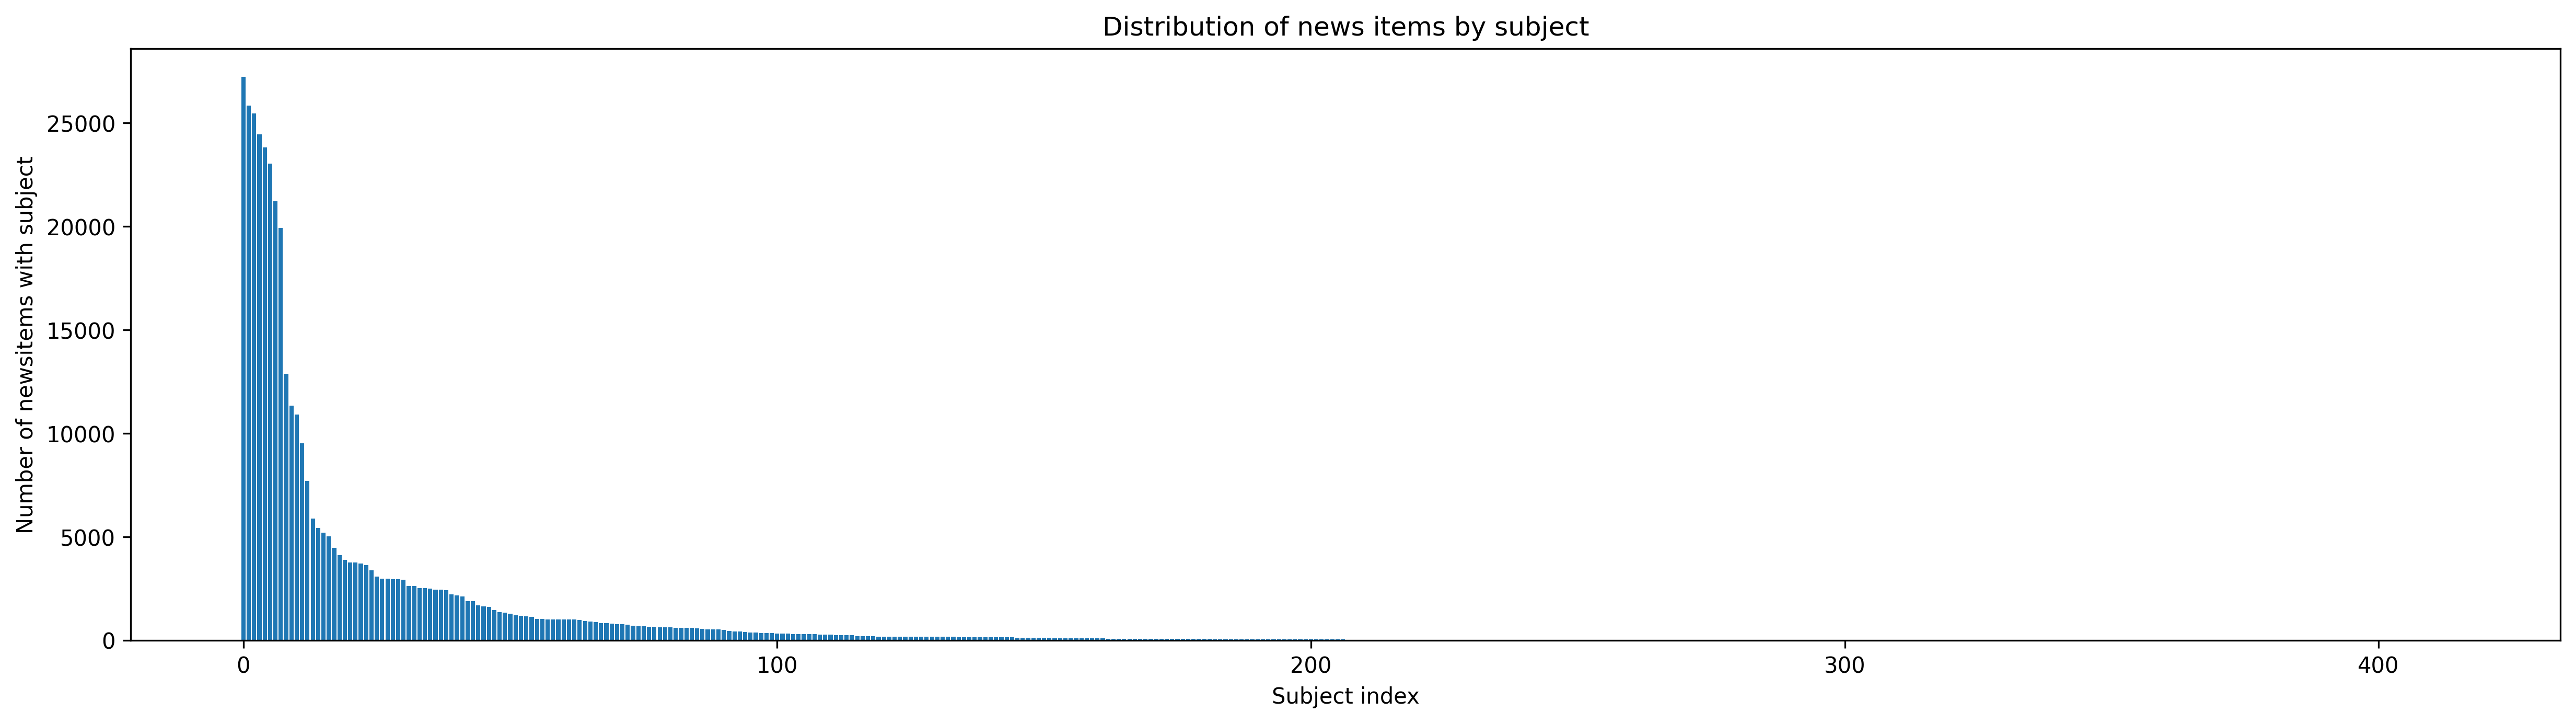
\includegraphics[scale=0.35]{distribution_news_item_subject}}
        \caption{\textit{Distribution of news items by subject}}
      \end{figure}

      \begin{figure}
        \centerline{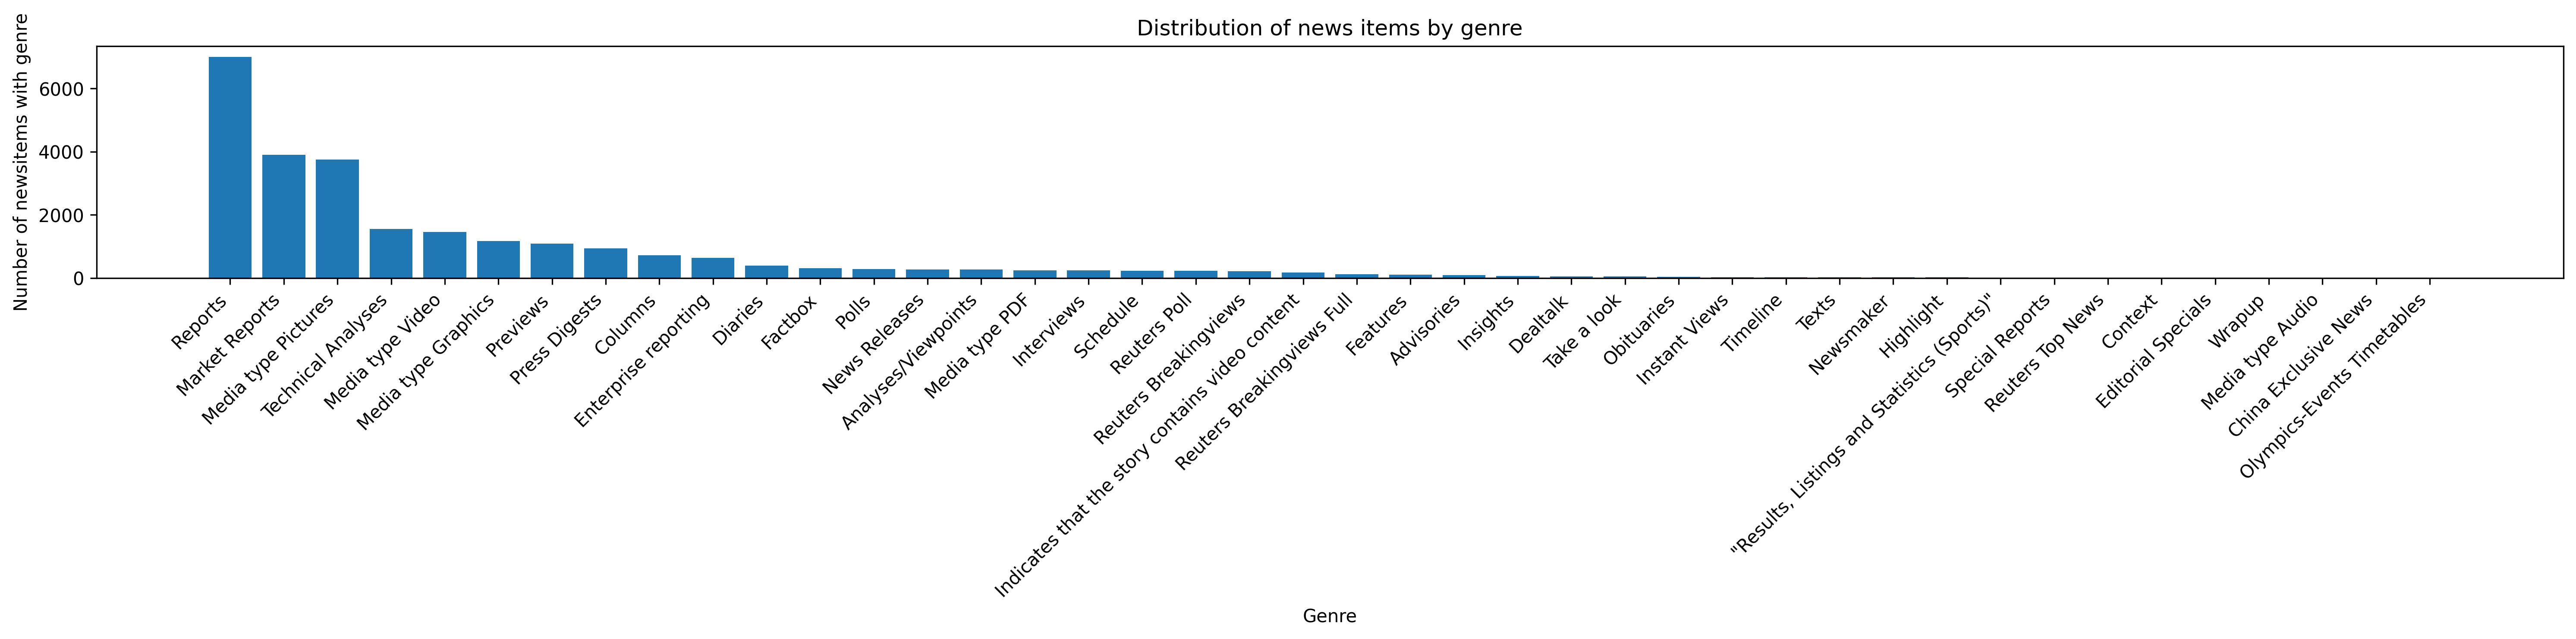
\includegraphics[scale=0.3]{distribution_news_item_genre}}
        \caption{\textit{Distribution of news items by genre}}
      \end{figure}

      }
    \end{itemize}

    \subsubsection{Challenges}
    Cleaning this dataset presented a few unique challenges, which will be considered in the NLP section below.
    \begin{itemize}
      \item{This corpus included some XML documents with unique encoding issues between UTF-8 encoding and plain text. For example, some of the XML documents\footnote{tag:reuters.com,2019:newsml\_CqtHM2P1a} included Tweets with emojis. A future effort could handle such emojis more gracefully. Furthermore, some apostrophes were transformed \footnote{For example, headline ``BREAKINGVIEWS-Carmakers,\"A\^o antitrust probe is more smoke than fire'' (tag:reuters.com,2019:newsml\_L2N25X0YW).}
      }
      \item{Some documents include table-formatted text, with many spaces meant to be rendered in a monospace format. In this case, a simple logic to consider a single space as a word boundary is not correct.\footnote{For example, item tag:reuters.com,2019:newsml\_L3N2602HC:991614233 should not be considered to have 76,783 words. It has 294,233 spaces when counting all whitespace, but this is a table-formatted item, not a long piece of text.}}
      \item{Some documents are incredibly long direct quotations transcribed from an event. These should be handled differently than other news reports.\footnote{For example, item tag:reuters.com,2019:newsml\_CqtYP8GSa:1548902168.XML is a full transcript of a committee hearing on US-China relations.}}
    \end{itemize}

    \subsubsection{Graph Database Ingestion}

    Finally, the CSVs were combined and ingested into Neo4g as a graph database. Cypher queries were run to ingest the primary metadata from each cleaned XML news item into Neo4j as a property graph with initial relationships (\textit{\textbf{Demo file available on Github}}\footnote{\lstinline{04_csvs_to_neo4j.cypher} (\href{https://github.com/Birkbeck/msc-data-science-project-2020_21---files-heychrisek/}{full code on Github})}). After running these Cypher queries, a prototype knowledge graph is available for meaningful queries and initial information retrieval (see\hyperref[sec:DataSetEvaluation]{``Data Evaluation''} below). This step uses Neo4j, Cypher, and APOC to load the cleaned CSV, create Neo4j nodes for each NewsItem, Subject, and Genre, add properties to the nodes, and create \lstinline{-[:HAS_GENRE]->} and \lstinline{-[:HAS_SUBJECT]->} relationships.


  \subsection{Data Evaluation}
  \label{sec:DataSetEvaluation}

  With the data sourcing, cleaning, and graph database ingestion complete, we can evaluate the raw data and begin to see the practical value of a knowledge graph in terms of information retrieval.

  At a basic level, the overall shape of the data and graph become clear. As shown in \textit{Table 2} and \textit{Table 3}, nearly 60,000 nodes are now available in the Neo4j graph database. Furthermore, there is interesting variance in the number of relationships per node, while keeping the properties per node constant across all NewsItems, Genres, and Subjects.


  \begin{table}
    \begin{tabular}{ |p{3cm}||p{2cm}|p{7cm}|  }
    \hline
    \multicolumn{3}{|c|}{Neo4j Knowledge Graph Nodes: high-level view of graph DB schema} \\
    \hline
    Node (Label)& Count &Properties\\
    \hline
    NewsItem&59,542&guid, filename, headline, slugline, datetime, genres, bodyLengthWords, subjects, description, bodyLengthChars, bodyLengthCharsNonWhitespace\\
    \hline
    Subject&414&category, subject, wikidataURL, wikipediaURL\\
    \hline
    Genre&42&genre\\
    \hline
    \end{tabular}
    \caption{\textit{Initial Knowledge Graph overview}}
  \end{table}

  \begin{table}
    \begin{lstlisting}
    MATCH (n)
    WITH labels(n) as labels, size(keys(n)) as props, size((n)--()) as degree
    RETURN
    DISTINCT labels,
    count(*) AS NumNodes,
    avg(props) AS AvgNumPropPerNode,
    min(props) AS MinNumPropPerNode,
    max(props) AS MaxNumPropPerNode,
    avg(degree) AS AvgNumRelationships,
    min(degree) AS MinNumRelationships,
    max(degree) AS MaxNumRelationships
    \end{lstlisting}

    \begin{tabular}{ |p{2cm}|p{1cm}|p{1.5cm}|p{1.5cm}|p{1.5cm}|p{1.5cm}|p{1.5cm}|p{1.5cm}| }
    \hline
    labels&Num-Nodes&AvgNum-PropPer-Node&MinNum-PropPer-Node&MaxNum-PropPer-Node&AvgNum-Relation-ships&MinNum-Relation-ships&MaxNum-Relation-ships\\
    \hline
    [``NewsItem'']&59542&11&11&11&7.6&0&94\\
    \hline
    [``Genre'']&42&1&1&1&618.3&1&7250\\
    \hline
    [``Subject'']&415&5&5&5&1021.1&0&27250\\
    \hline
    \end{tabular}

    \caption{\textit{Cypher query\protect \footnotemark to inventory initial nodes and relationships in the knowledge graph}}
  \end{table}

  \footnotetext{\url{https://neo4j.com/developer/kb/how-do-i-produce-an-inventory-of-statistics-on-nodes-relationships-properties/}}
  
  More significantly, at this point the knowledge graph's practical value begins to become evident, as some human-interpretable queries are now possible, which were not originally possible with the raw data. Whereas the unstructured collection of semi-structured XML documents could not be queried, now we can present meaningful queries over the dataset, including the following (\textit{\textbf{Demo file available on Github}}\footnote{\lstinline{05_query_kg.cypher} (\href{https://github.com/Birkbeck/msc-data-science-project-2020_21---files-heychrisek/}{full code on Github})}).

  \begin{itemize}
    \item{Finding all news items that have two specific subjects or all items that have more than a certain number of genre or subject relationships (see \textit{Figure 3}).}
    \item{Finding the shortest news items and longest news items by length in characters (see \textit{Figure 4}).}
    \item{Finding the subjects and genres assigned to the most items (see \textit{Figure 5}). Note that these figures confirm what was already discovered in the distribution findings of \textit{Figure 1} and \textit{Figure 2}.}
    \item{Finding the shortest path between two items, perhaps to quickly see what some news stories have in common (see \textit{Figure 6}).}
  \end{itemize}

  \begin{figure}
    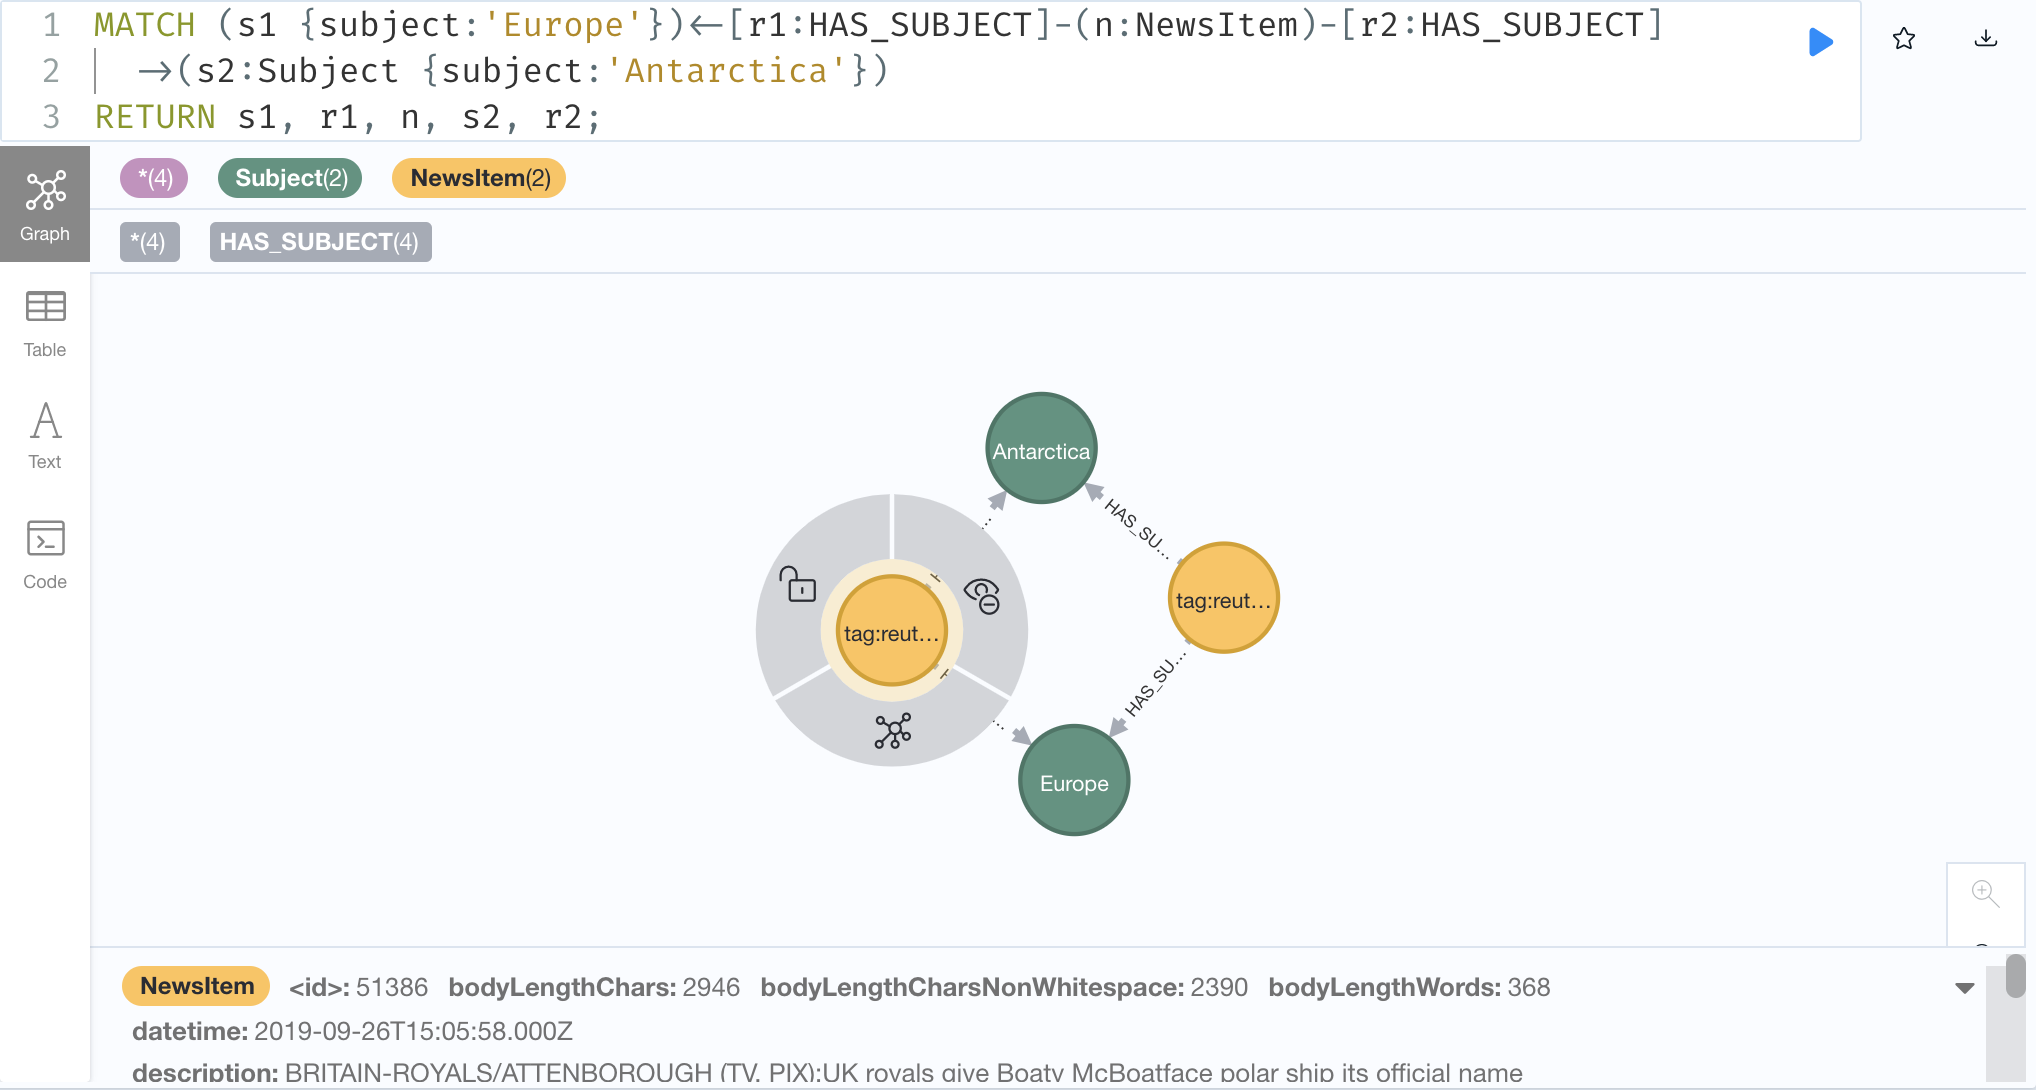
\includegraphics[scale=0.2]{00-news-items-antarctica-europe}
    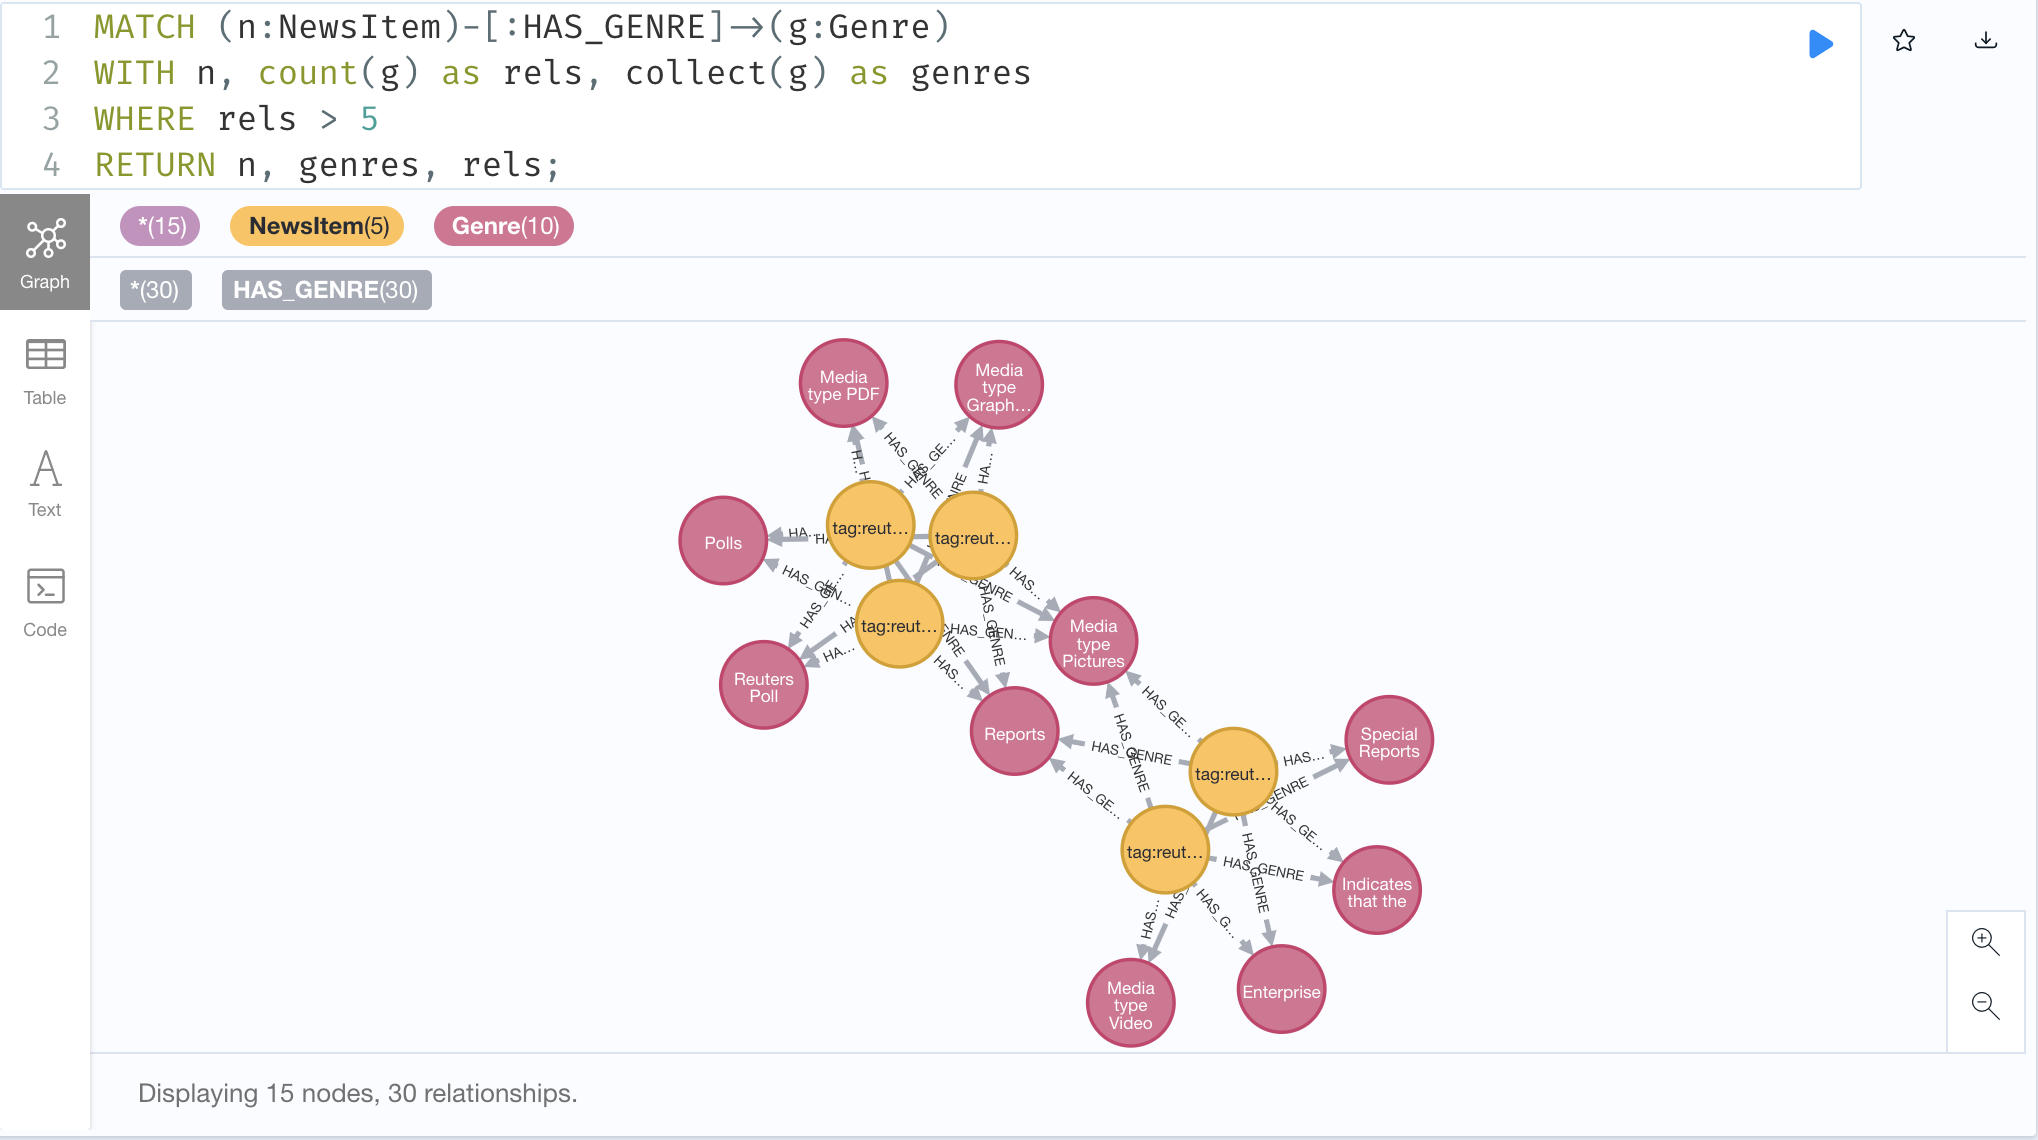
\includegraphics[scale=0.2]{00-news-items-more-than-five-genres}
    \caption{\textit{Knowledge graph Cypher queries: subject and genre relationships)}}
  \end{figure}

  \begin{figure}
    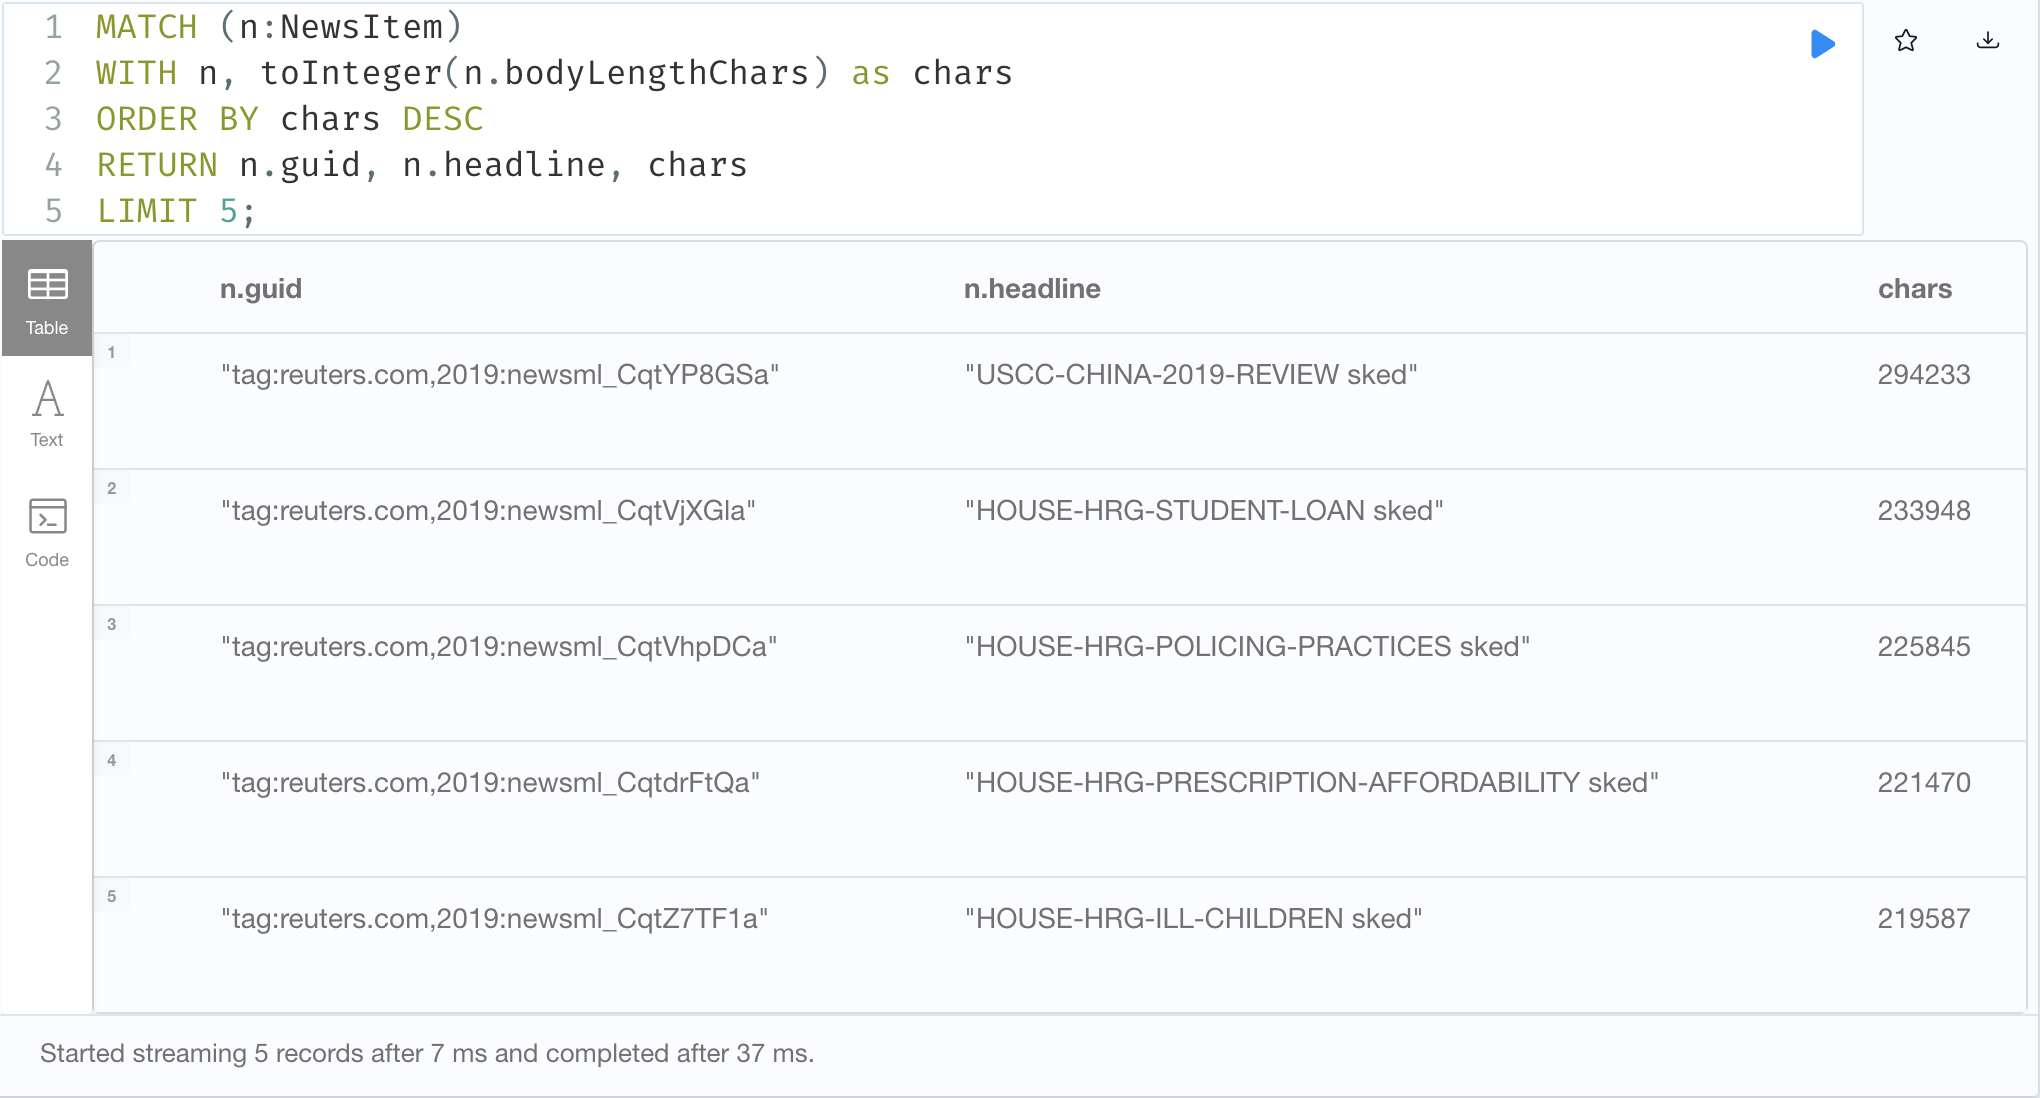
\includegraphics[scale=0.2]{01-longest-items}
    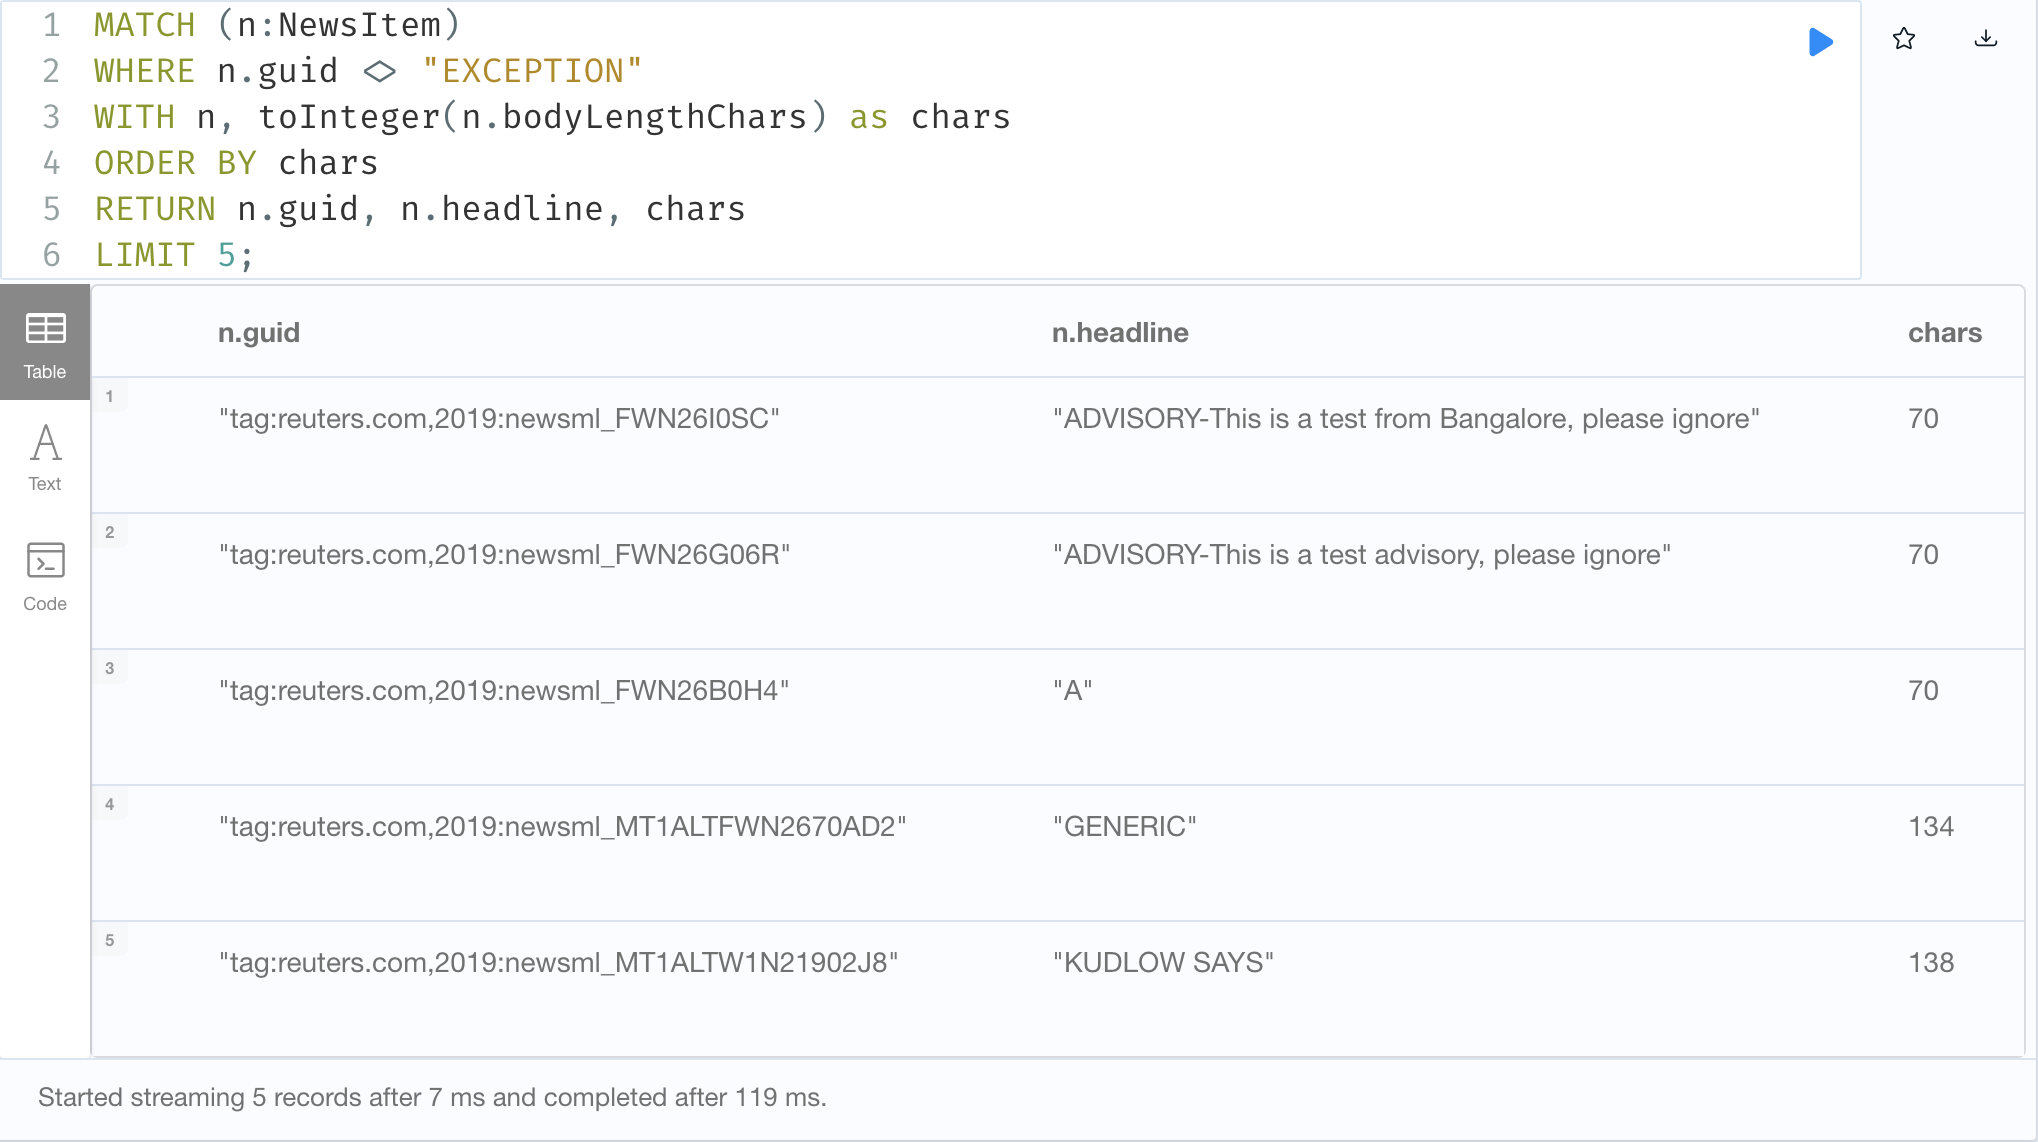
\includegraphics[scale=0.2]{01-shortest-items}
    \caption{\textit{Knowledge graph Cypher queries: shortest and longest news text}}
  \end{figure}

  \begin{figure}
    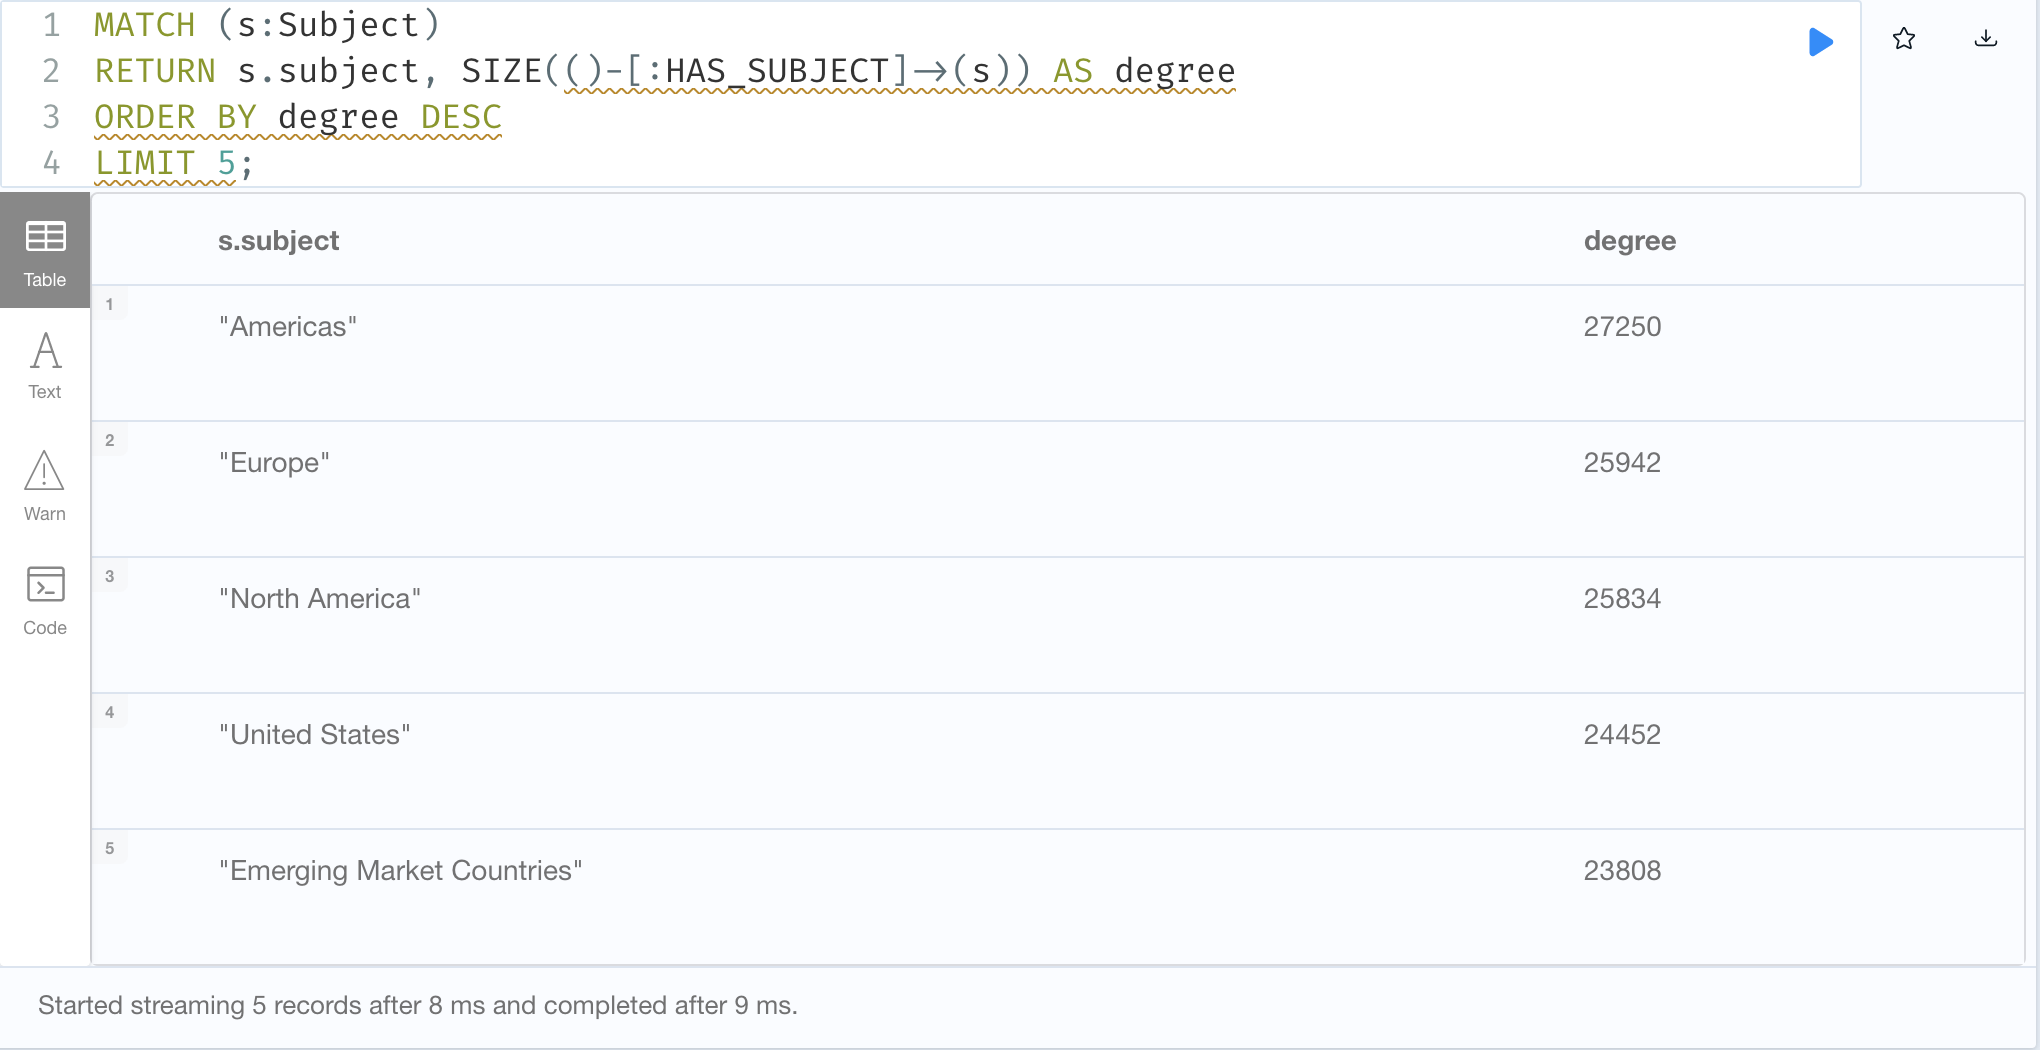
\includegraphics[scale=0.2]{02-subjects-with-most-items}
    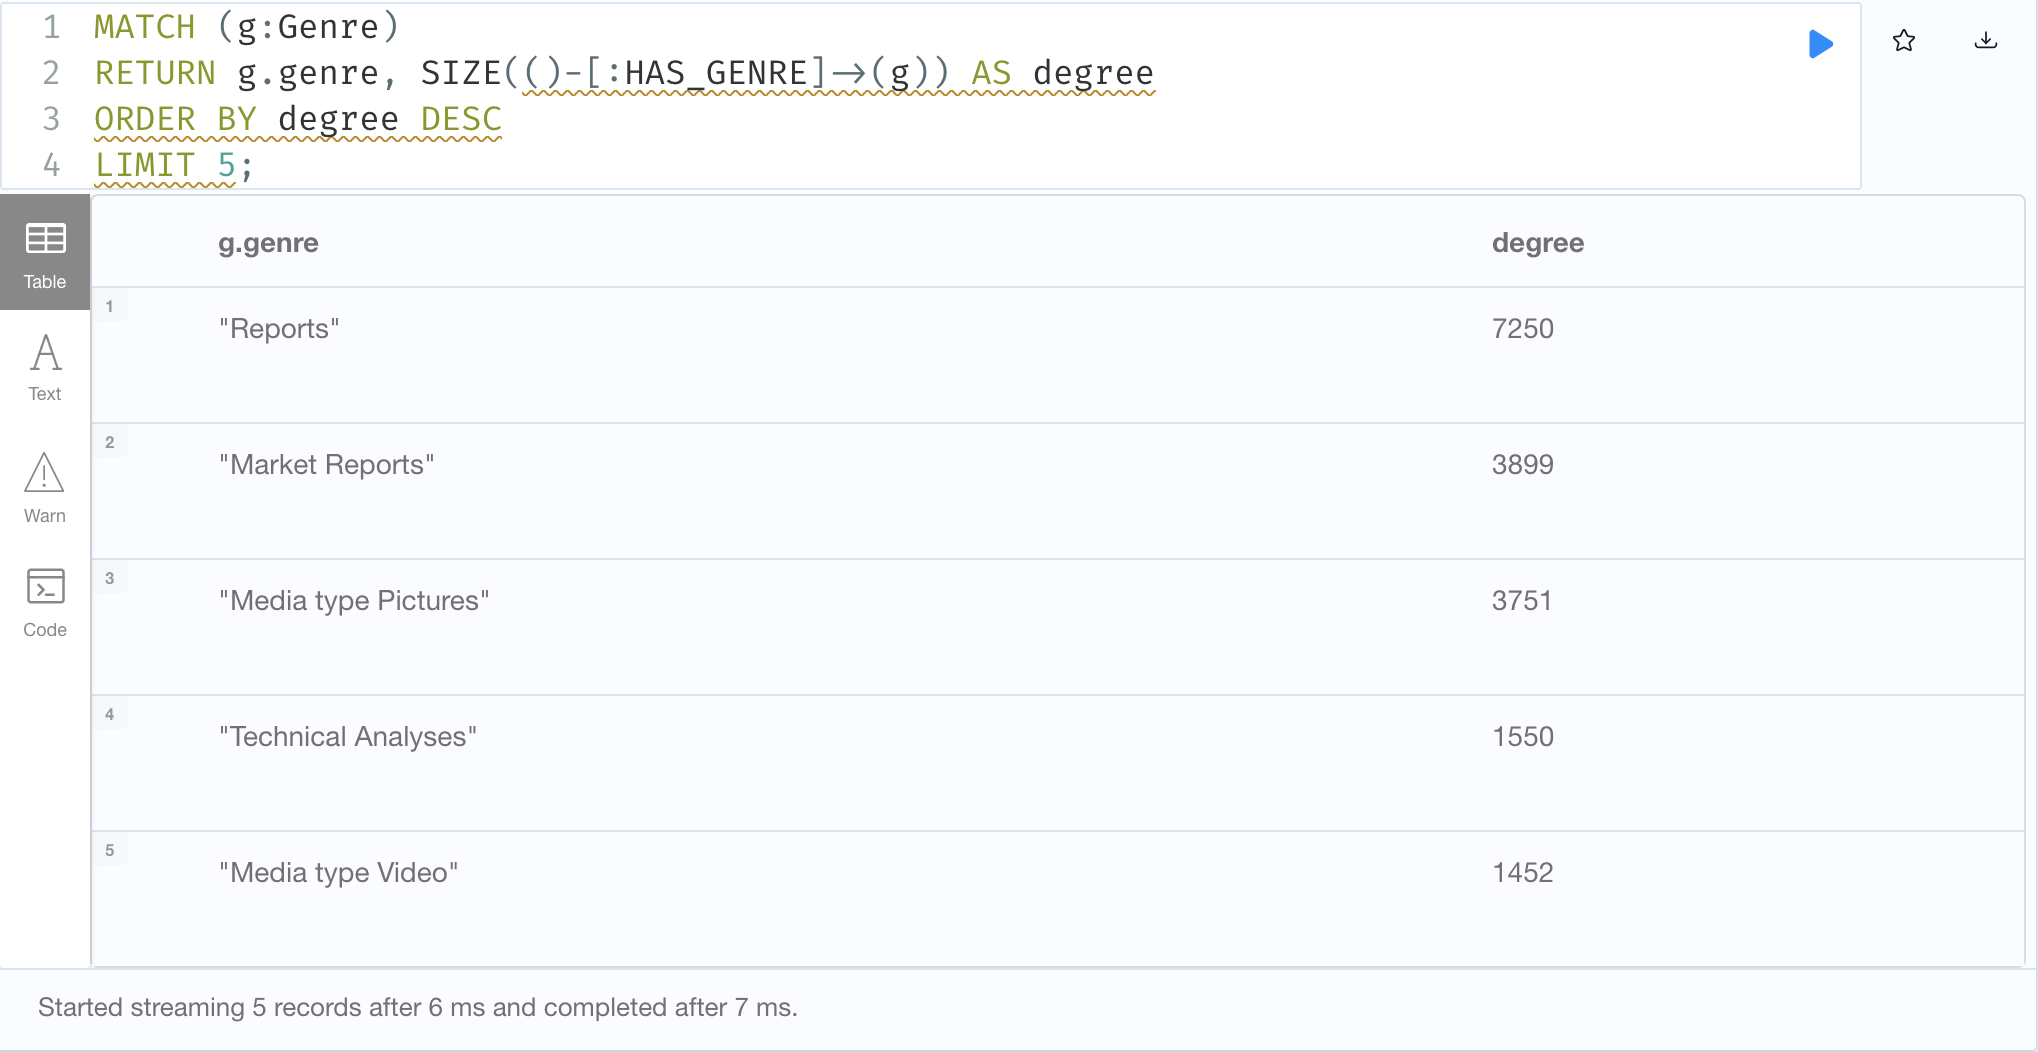
\includegraphics[scale=0.2]{02-genres-with-most-items}
    \caption{\textit{Knowledge graph Cypher queries: subjects and genres with most items}}
  \end{figure}

  \begin{figure}
    \centerline{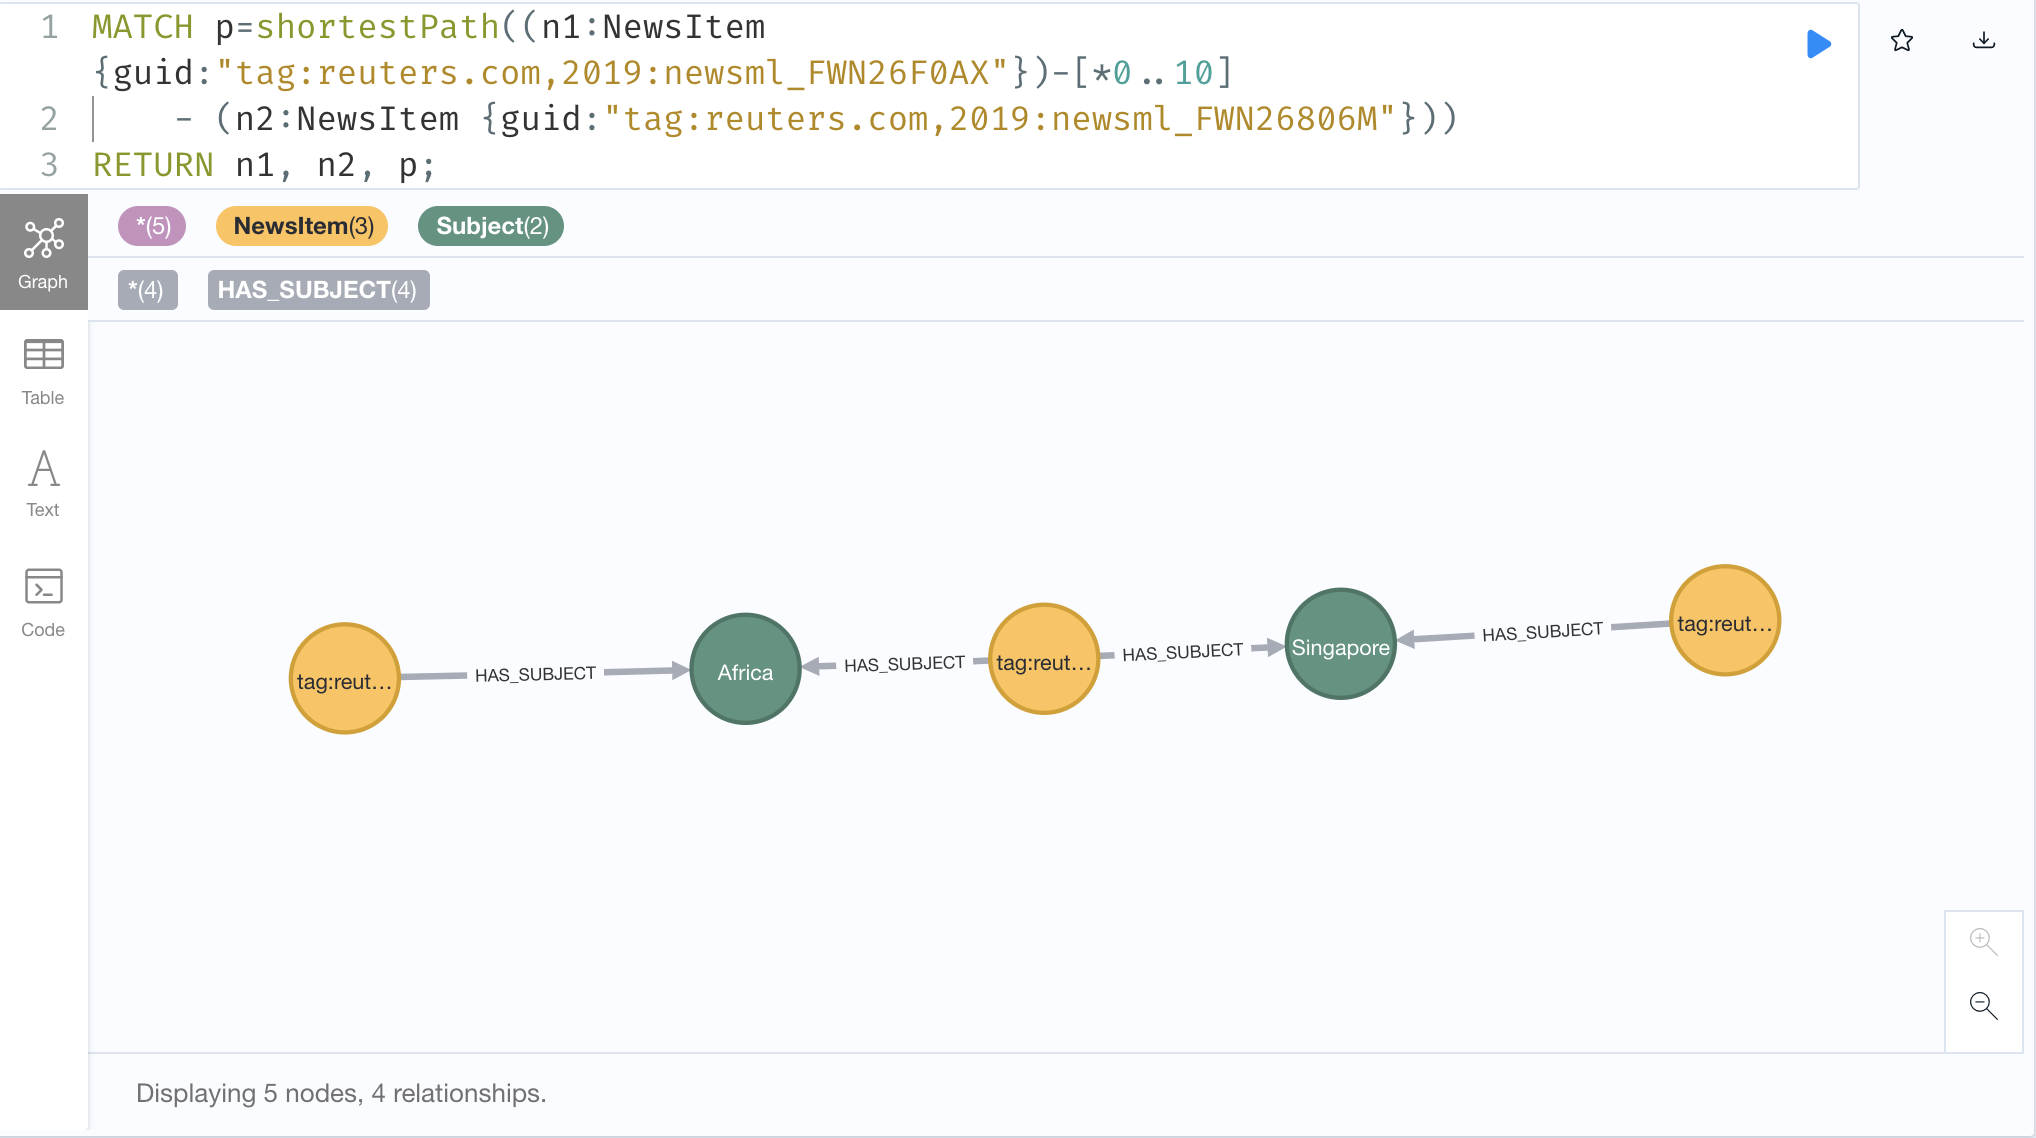
\includegraphics[scale=0.2]{03-shortest-path}}
    \caption{\textit{Knowledge graph Cypher queries: shortest path}}
  \end{figure}


\section{Knowledge Graph Design and Enhancement}

Building on the domain-sepcific knowledge graph of news items from the previous sections, the analysis now focuses on enhancements to the knowledge graph. This includes (1) semantic enhancements using ontologies and linked data; (2) NLP enhancements to extract entities and other meaning from the English language text; and (3) network analysies around centrality, clustering, and betweenness. It draws guidance and technical examples from Neo4j's developer guides\footnote{\url{https://neo4j.com/developer/}}, including the Neo4j knowledge graph tutorial\cite{neo4j-kg-tutorial}.

  \subsection{Semantic Enhancements}

  Neo4j has a useful plugin called neosemantics (n10s), which ``enables the use of RDF and its associated vocabularies like (OWL,RDFS,SKOS and others) in Neo4j'' \footnote{\url{https://neo4j.com/labs/neosemantics/}}. This makes n10s a suitable technology for semantic enhancements of the news knowledge graph.

  For this knowledge graph, Wikidata\footnote{\url{https://www.wikidata.org/}} was chosen as the knowledge base to link with the published news documents. After reflecting on the content of the Reuters news items, it became clear that a few resource types are commonly present in news items:
  \begin{itemize}
    \item{Geography (countries, cities)}
    \item{People (politicians, athletes)}
    \item{Organisations (political parties, companies)}
  \end{itemize}

  SPARQL queries can find the Wikidata category for each of these and recursively identify the subcategories. By importing these categories and subcategories in an RDF subject-predicate-object format with n10s, the Neo4j knowledge graph can represent the relationships between parent/child categories and instances of specific categories (\textit{\textbf{Demo file available on Github}}\footnote{\lstinline{06a_kg_nlp_entities.cypher} and \lstinline{06b_SPARQL-endpoints.txt} (\href{https://github.com/Birkbeck/msc-data-science-project-2020_21---files-heychrisek/}{full code on Github})}).

  For example:
  \begin{lstlisting}
    WITH "https://query.wikidata.org/sparql?query=..." AS uri
    CALL n10s.rdf.import.fetch(uri, "Turtle", { headerParams: { Accept: "application/x-turtle" } })
    YIELD terminationStatus, triplesLoaded, triplesParsed, namespaces, callParams
    RETURN terminationStatus, triplesLoaded, triplesParsed, namespaces, callParams;

    MATCH path = (c:Category {name: "republic"})<-[:SUB_CAT_OF*]-(child)
    RETURN path
    LIMIT 25;
  \end{lstlisting}

  \begin{figure}
    \centerline{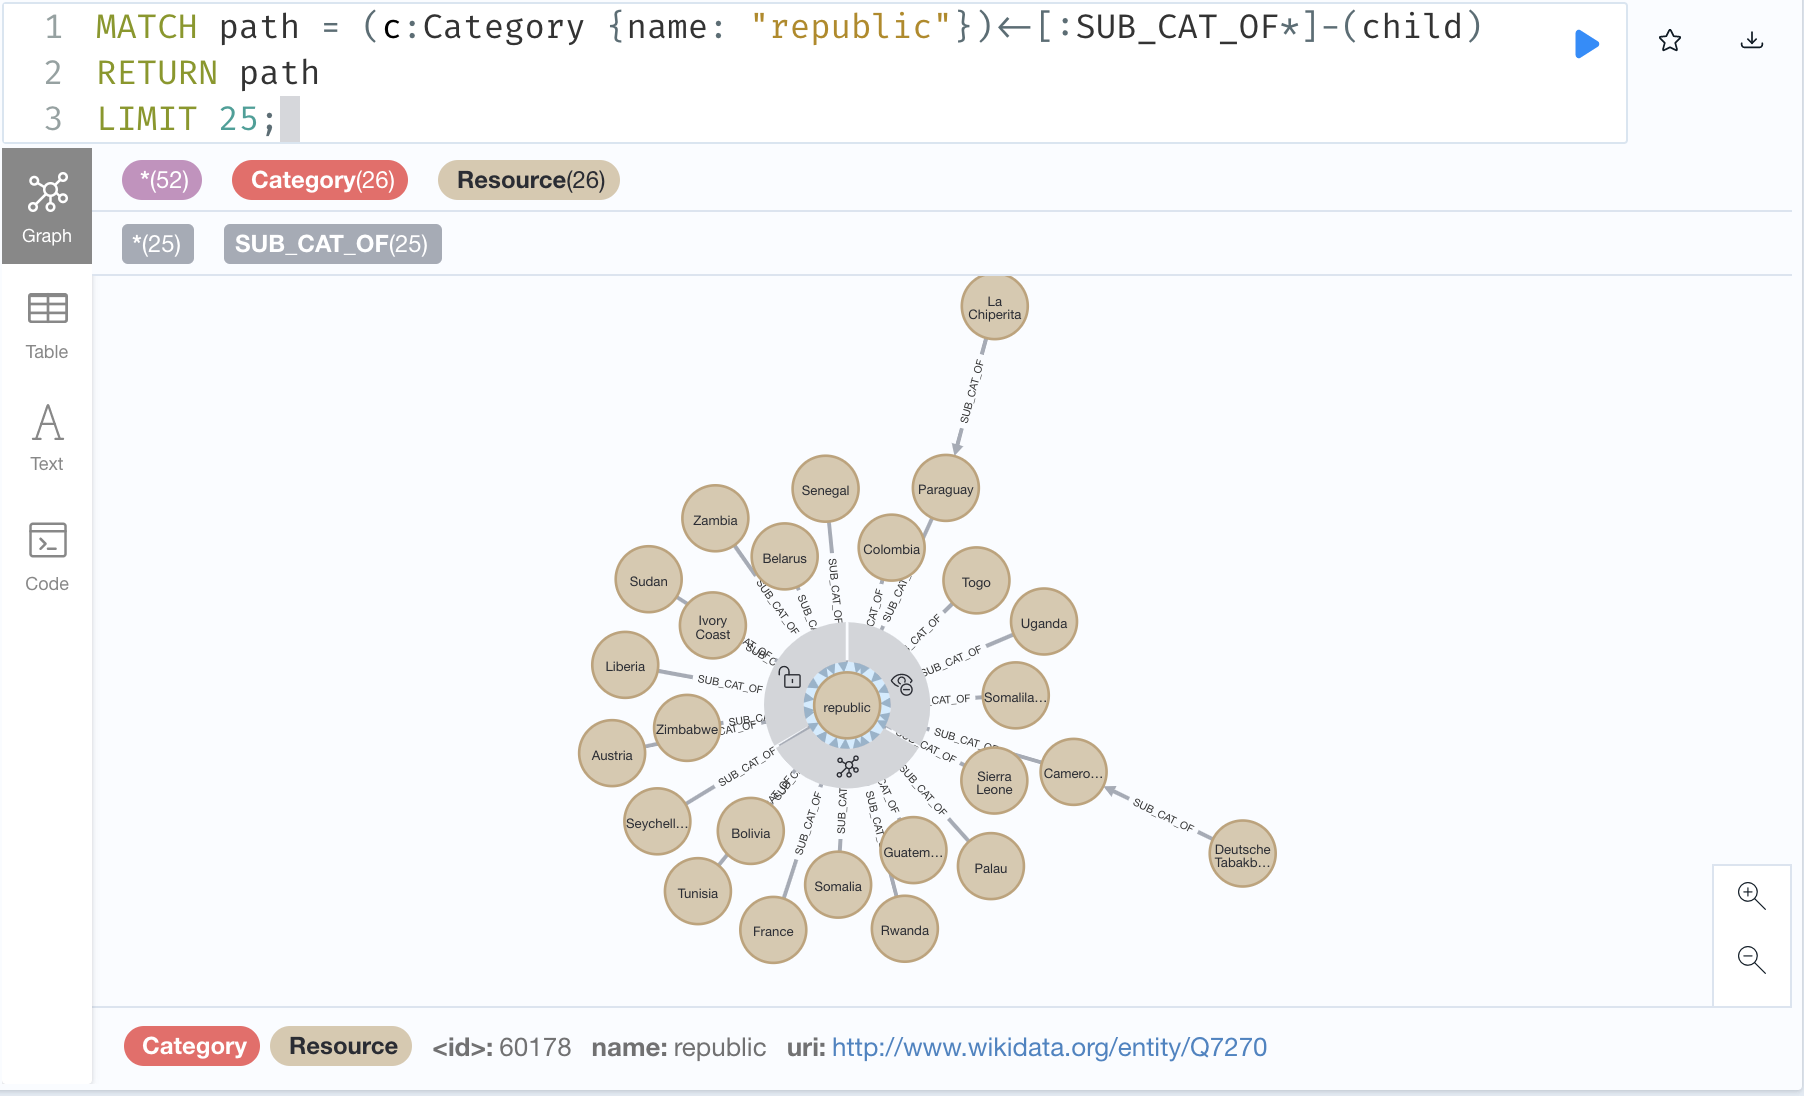
\includegraphics[scale=0.5]{category-republic.png}}
    \caption{\textit{Countries which are instances of republic}}
  \end{figure}

  This provides a foundation of knowledge via Wikidata's ontology, which can now be connected to facts from the news items via natural language processing and entity extraction.

  \subsection{Natural Language Processing}

  The APOC plugin enables Neo4j Cypher queries to use the Google Cloud Platform's entity extraction procedures\footnote{\url{https://neo4j.com/labs/apoc/4.1/nlp/gcp}}, by providing a \lstinline{nodeProperty} parameter, in this case \lstinline{body} for the news item's text body (\textit{\textbf{Demo file available on Github}}\footnote{\lstinline{06a_kg_nlp_entities.cypher} (\href{https://github.com/Birkbeck/msc-data-science-project-2020_21---files-heychrisek/}{full code on Github})}).

  By running entity extraction over each news item's text body, which takes approximately 10 hours for all 59,542 items, we can now see entities for a given news item. For example, a news item about the Gap clothing company may have entities United States, Gap, and Sephora (see ``Figure 13'').

  \begin{figure}
    \centerline{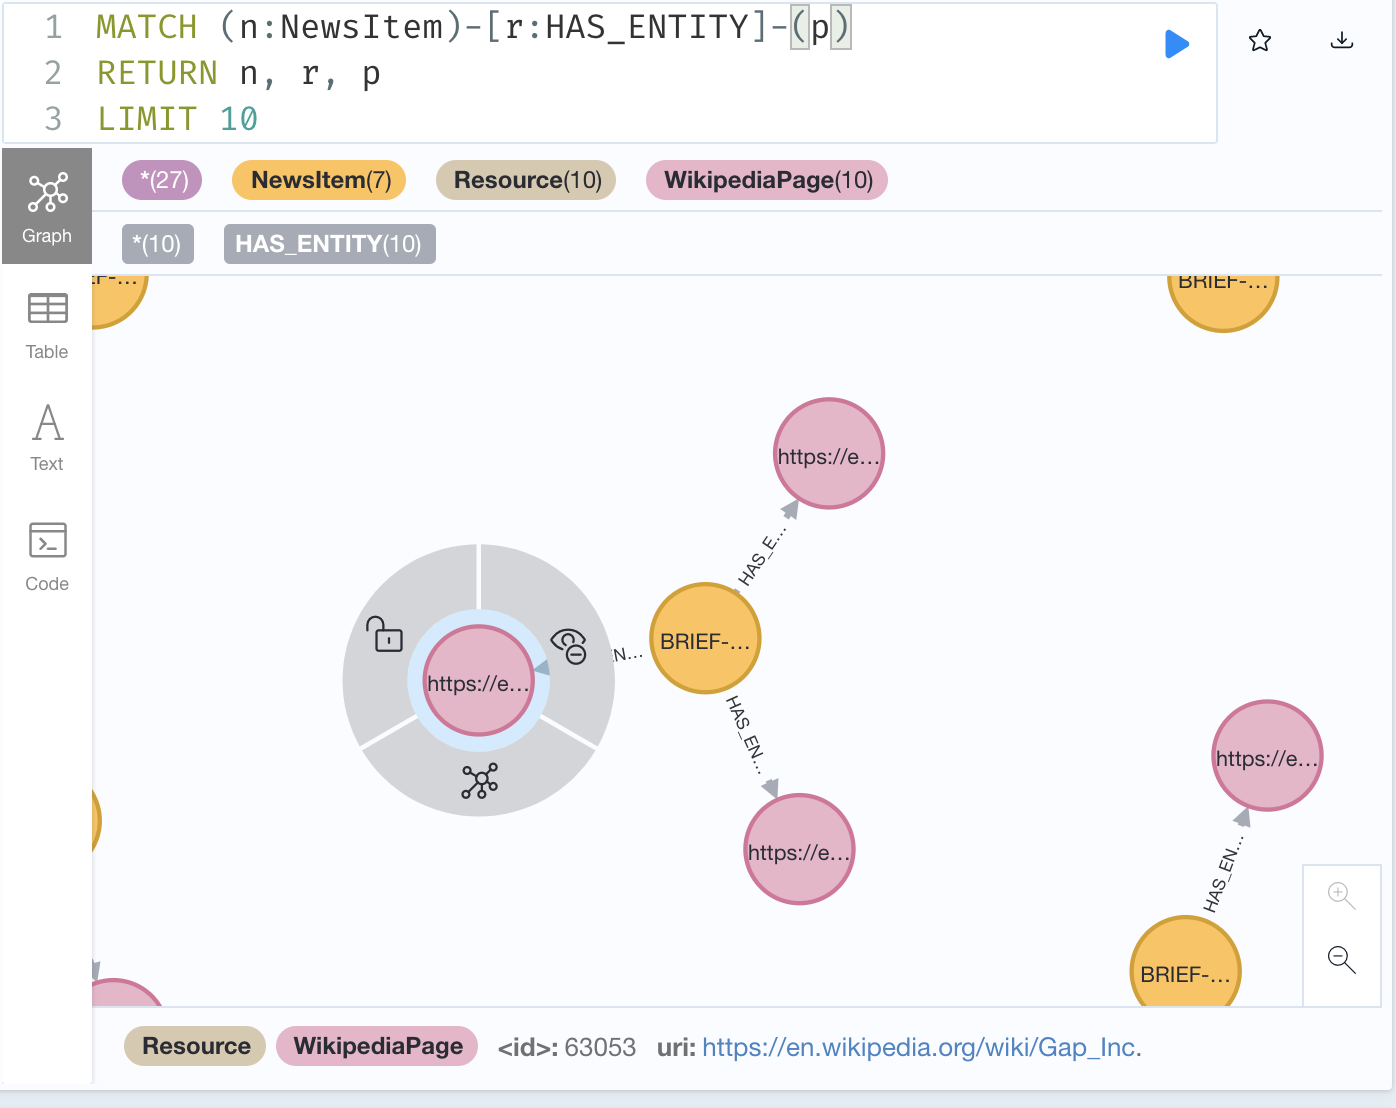
\includegraphics[scale=0.5]{has-entity.png}}
    \caption{\textit{\lstinline{(n:NewsItem)-[:HAS_ENTITY]->(p:WikipediaPage)}}}
  \end{figure}

  This entity analysis procedure was quite successful, extracting 39,884 entities that have Wikipedia pages and 506,283 new \lstinline{-[:HAS_ENTITY]->} relationships, since many news items have the same entity. In fact, the most common entity is the United States, which appears in 16,694 news items, or 28\% of all news items (see ``Figure 14'').  


  \begin{figure}
    \centerline{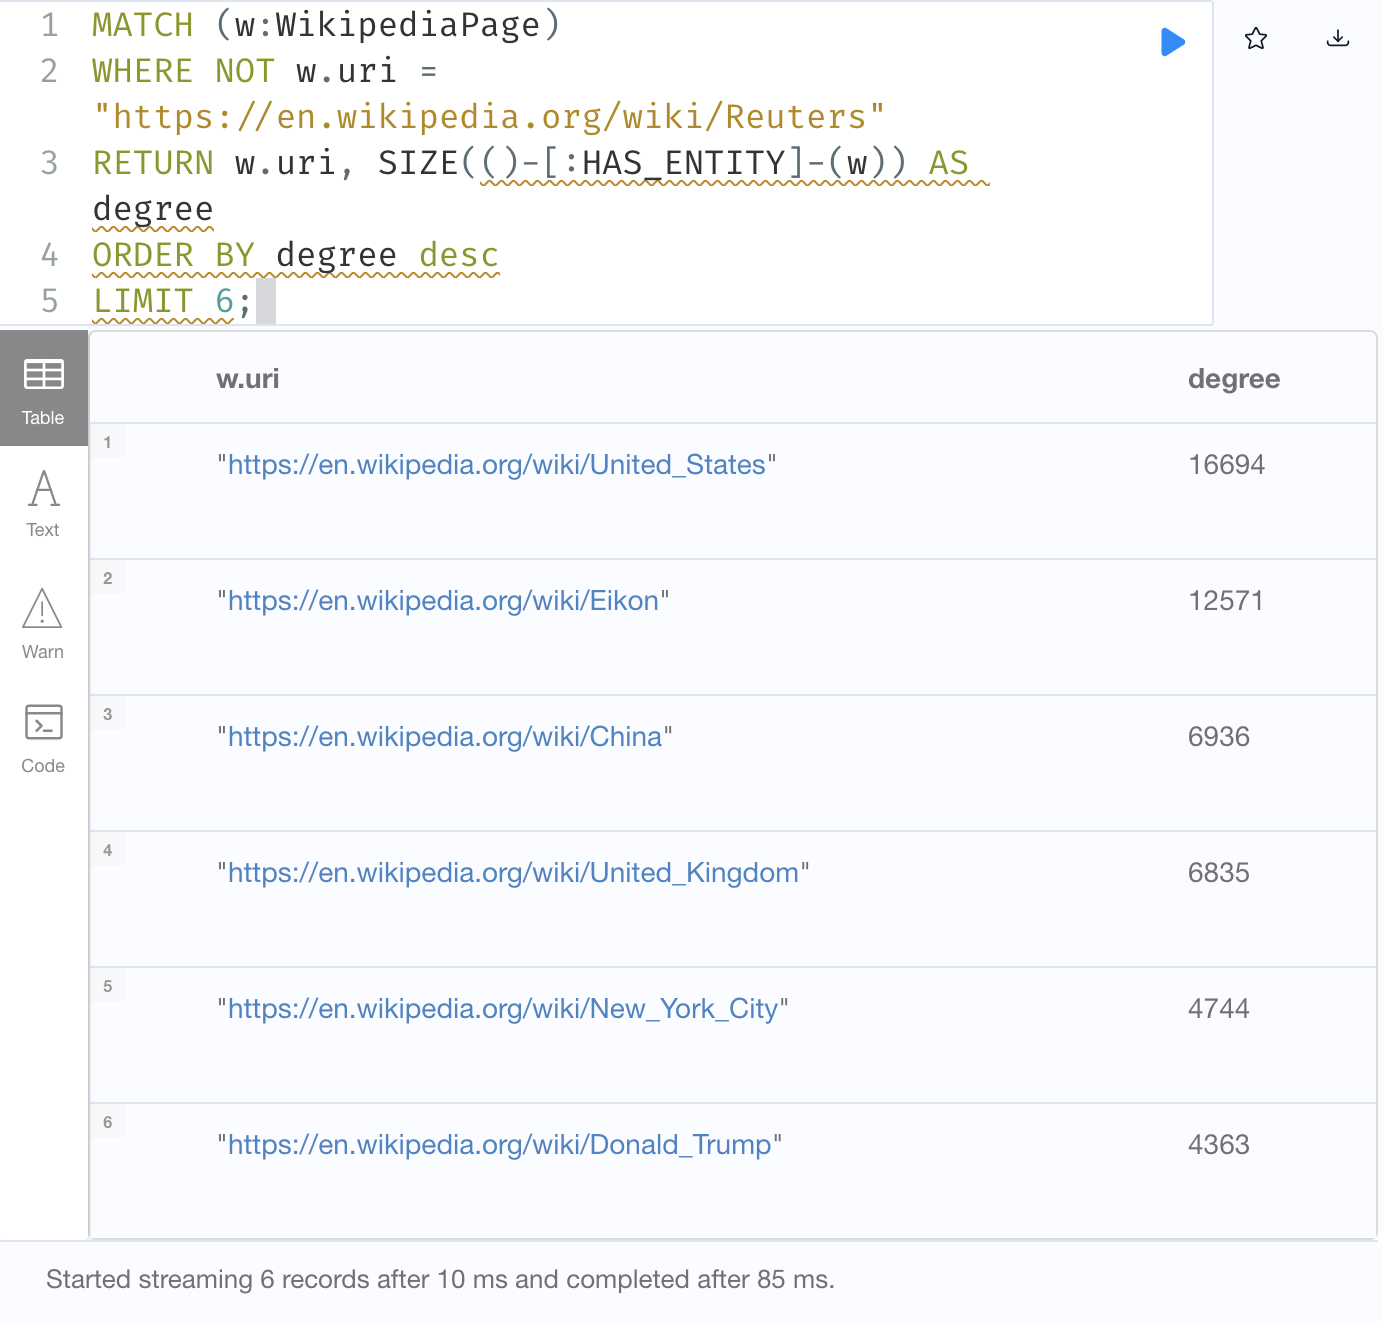
\includegraphics[scale=0.5]{highest-degree-entities.png}}
    \caption{\textit{Entities that appear in the most news items}}
  \end{figure}

  \section{Evaluation}

  It is clear that the data pipeline and resulting knowledge graph perform well at a scale of tens of thousands of news items. Furthermore, the semantic enhancement is a success, as demonstrated by the nearly 40,000 Wikipedia pages that are now linked as extracted entities in the news knowledge graph. Compared to the original ``Table 3'' above, we can see that additional categories and entities are now available:

  \begin{table}
    \begin{tabular}{ |p{2cm}|p{1cm}|p{1.5cm}|p{1.5cm}|p{1.5cm}|p{1.5cm}|p{1.5cm}|p{1.5cm}| }
    \hline
    labels&Num-Nodes&AvgNum-PropPer-Node&MinNum-PropPer-Node&MaxNum-PropPer-Node&AvgNum-Relation-ships&MinNum-Relation-ships&MaxNum-Relation-ships\\
    \hline
    [``NewsItem'']&59542&13&12&13&16.1&0&458\\
    \hline
    [``Genre'']&42&1&1&1&618.3&1&7250\\
    \hline
    [``Subject'']&415&5&5&5&1021.1&0&27250\\
    \hline
    [``Resource'', ``Category'']&6982&2&2&2&4.8&1&1712\\
    \hline
    [``Resource'', ``WikipediaPage'']&39884&1&1&1&12.8&1&43154\\
    \hline
    \end{tabular}

    \caption{\textit{Cypher query\protect \footnotemark to inventory final nodes and relationships in the knowledge graph after semantic enhancements and NLP entity extraction}}
  \end{table}

  Furthermore, the practical value has already been demonstrated in the ``Benefits and Use Cases'' section above. Journalistic users and general knowledge graph practitioners can use this pipeline to generate a knowledge graph or can use the resulting knowledge graph to enhance work product in the media space.

  One area for improvement is de-coupling the data extraction pipeline from the news domain and NewsML XML structure. For example, the de-couple this as a reusable pipeline for any domain and XML structure, the following interfaces need to be better defined:
  \begin{itemize}
    \item{\textit{XML mapping} - As mentioned in ``4.2.2. Extract XML Properties'' above, the current script hardcodes the selection of news-relevant properties via NewsML xpath locators. This would need to be abstracted to enable application of the pipeline to a new XML structure.}
    \item{\textit{SPARQL endpoints} - As described in ``5.1 Semantic Enhancements'', SPARQL endpoints enabled the knowledge graph to link to Wikidata categories in areas such as countries, cities, politicians, and athletes. Applied to another domain, this pipeline would need an interface by which a user could input SPARQL endpoints of their own choosing.}
    \item{\textit{GCP entity analysis API} - As described in ``5.2 Natural Language Processing'', the Google Cloud Platform API for entity analysis was run against each news item's text body via the \lstinline{body} property. Other users may create a data model where entity extraction should run against a different property, so this coupling to text body should be abstracted.}
  \end{itemize}

  Finally, evaluating against the aims and objectives outlined in the ``Research Problem'' section above, this project has successfully accomplished its aims of designing and implementing an information retrieval system in the news domain, while validating the use of technologies including knowledge graphs, ontologies, linked data, and natural language processing. These aims were accomplished by completing the concrete objectives of a software specification, data extraction pipeline, knowledge graph prototype, and experimental application of additional technologies.

  This effort also raises additional questions and areas for future research, which are outlined in the following ``Conclusion'' section.

  % \subsection{Interpretability}
  % \subsection{Others...confusion matrix, predictions, clustering, betweenness, etc.}

\section{Conclusions}

This project exhibited the viability of applying semantic technologies and natural language processing to create a knowledge graph in the news domain. Beyond the practical outcomes that are now possible via graph queries, the resulting knowledge graph is especially meaningful in terms of human interpretability.

While much research in artificial intelligence and machine learning still suffers from a black box problem, by which ``we typically have little understanding on why AI systems make decisions or exhibit certain behaviors''\cite{rai2020explainable}, a knowledge graph enables very interpretable and human-understandable outcomes. AI and ML techniques can be applied to this news knowledge graph, and a human user would still be able to trace the path in the graph to understand the fundamental data.

That said, this is a major area for additional focus. Knowledge graphs have potential for combining with machine learning, via graph embeddings or statistical relational models\cite{wang2017knowledge}\cite{nickel2015review}.

The efforts of this project also set a foundation for additional application of algorithms and graph analysis. For example, this analysis demonstrated some possibilities for querying news items by similarity and generating recommendations. Other algorithms can be applied\footnote{\url{https://neo4j.com/docs/graph-data-science/current/algorithms/}}, including network analyses for determining the centrality or importance of graph nodes\footnote{\url{https://neo4j.com/docs/graph-data-science/current/algorithms/centrality/}} or link prediction algorithms for determining closeness of two distinct nodes and predicting new relationships\footnote{\url{https://neo4j.com/docs/graph-data-science/current/algorithms/linkprediction/}}. A future effort would apply such algorithms and evaluate their suitability for knowledge graphs in the news domain.

\newpage

\section{Appendix}

In lieu of an appendix, all code has been made available in a Github repository: \url{https://github.com/Birkbeck/msc-data-science-project-2020_21---files-heychrisek}.

Readers are encouraged to view the \textbf{demo} section of the repository, where they can follow instructions to build a knowledge graph using a sample of news items:
\begin{itemize}
  \item{Demo README: \url{https://github.com/Birkbeck/msc-data-science-project-2020_21---files-heychrisek/tree/main/demo}}
  \item{Demo video: \url{https://youtu.be/w5ZIPvBq8NQ}}
\end{itemize}

\newpage

\bibliographystyle{abbrv}
\bibliography{project}

\end{document}
